% This must be in the first 5 lines to tell arXiv to use pdfLaTeX, which is strongly recommended.
\pdfoutput=1
% In particular, the hyperref package requires pdfLaTeX in order to break URLs across lines.

\documentclass[11pt,dvipsnames]{article}

% Remove the "review" option to generate the final version.
\usepackage[]{ACL2023}

% Standard package includes
\usepackage{times}
\usepackage{latexsym}

% For proper rendering and hyphenation of words containing Latin characters (including in bib files)
\usepackage[T1]{fontenc}
% For Vietnamese characters
% \usepackage[T5]{fontenc}
% See https://www.latex-project.org/help/documentation/encguide.pdf for other character sets

% This assumes your files are encoded as UTF8
\usepackage[utf8]{inputenc}

% This is not strictly necessary, and may be commented out.
% However, it will improve the layout of the manuscript,
% and will typically save some space.
\usepackage{microtype}

% This is also not strictly necessary, and may be commented out.
% However, it will improve the aesthetics of text in
% the typewriter font.
\usepackage{inconsolata}

\usepackage{multirow,hyperref}
\usepackage{graphicx}
\usepackage{diagbox}
\usepackage{booktabs}
% \usepackage{subfigure}
\usepackage{xspace}
\usepackage[ruled, vlined, linesnumbered]{algorithm2e}
% \usepackage{algorithm}
% \usepackage[linesnumbered,ruled,vlined]{algorithm2e}
% \usepackage{amssymb}
\usepackage{bbding}
\usepackage{threeparttable}
\usepackage{amsmath}
\usepackage{adjustbox}
\usepackage{listings}
\usepackage[T1]{fontenc}
\usepackage{semantic}
\usepackage{newfloat}
\usepackage{framed}
\usepackage{threeparttable}

\newtheorem{definition}{\bf Definition}
\newtheorem{theorem}{\bf Theorem}
\newtheorem{lemma}{\bf Lemma}
\newtheorem{assumption}{\bf Assumption}
\newtheorem{remark}{\bf Remark}
\newtheorem{proposition}{\bf Proposition}
\newtheorem{corollary}{\bf Corollary}
\newtheorem{property}{\bf Property}
\newtheorem{problem}{\bf Problem}
\newcommand{\e}[1]{\ensuremath{\times 10^{#1}}}
\newcommand{\ud}{\mathrm{d}}
\newcommand{\unsim}{\mathord{\sim}}
\newcommand{\tabincell}[2]{\begin{tabular}{@{}#1@{}}#2\end{tabular}}
\usepackage{makecell}

% \PassOptionsToPackage{prologue,dvipsnames}{xcolor}
% \usepackage[dvipsnames]{xcolor}

\usepackage{hyperref}
\hypersetup{
colorlinks=true,
linkcolor=blue,
filecolor=megenta
}



\newcounter{mydoublefinding}
\counterwithin*{mydoublefinding}{subsection}
\newenvironment{mydoublefinding}[2][]{%
\stepcounter{mydoublefinding}%
\begin{framed}%
\noindent\textbf{Findings #1.\themydoublefinding} #2%
\end{framed}}

\newcounter{myfindings}
\counterwithin*{myfindings}{section}
\newenvironment{myfindings}[2][]{%
\stepcounter{myfindings}%
\begin{framed}%
\noindent\textbf{Summary#1:} #2%
\end{framed}}

\usepackage{pifont}% http://ctan.org/pkg/pifont
\newcommand{\cmark}{\ding{51}}%
\newcommand{\xmark}{\ding{55}}%

\newcommand{\CodeIn}[1]{{\small\texttt{#1}}}


\DeclareFloatingEnvironment[fileext=frm,placement={!ht},name=Rules]{infrule}


\lstset{
    backgroundcolor = \color{yellow!10},    % 背景色:淡黄
    basicstyle = \ttfamily\footnotesize,           % 基本样式 + 小号字体
    rulesepcolor= \color{gray},             % 代码块边框颜色
    breaklines = true,                  % 代码过长则换行
    % numbers = left,                     % 行号在左侧显示
    % numberstyle = \small,               % 行号字体
    keywordstyle = \color{blue},            % 关键字颜色
    commentstyle =\color{gray!100},        % 注释颜色
    stringstyle = \color{red!100},          % 字符串颜色
    frame = shadowbox,                  % 用(带影子效果)方框框住代码块
    showspaces = false,                 % 不显示空格
    columns = fixed,                    % 字间距固定
    morekeywords = {as},                
    % 自加新的关键字(必须前后都是空格)
    deletendkeywords = {compile},    
    % 删除内定关键字;删除错误标记的关键字用deletekeywords删!
    escapeinside=``
}
\usepackage{algpseudocode}
\usepackage[normalem]{ulem}
\useunder{\uline}{\ul}{}

\newcommand\detector{VulLibGen}
% \newcommand\DETECTOR{DETECTOR}
\newcommand\vullib{VulLib}
% \newcommand\JAVADATA{JAVADATA}
% \newcommand\javadataone{JavaData-One}
% \newcommand\javadatazero{JavaData-Zero}
\newcommand\veracode{Veracode}
\newcommand\verajava{VeraJava}
\newcommand\veradata{Veracode}

\newcommand{\tianyu}[1]{\textcolor{blue}{Tianyu (TBD): #1}}

\newcommand{\xueqing}[1]{\textcolor{red}{Xueqing (TBD): #1}}

% If the title and author information does not fit in the area allocated, uncomment the following
%
%\setlength\titlebox{<dim>}
%
% and set <dim> to something 5cm or larger.

\title{VulLibGen: Generating Names of Vulnerability-Affected Packages via a Large Language Model}


\author{
  Tianyu Chen\textsuperscript{1}, Lin Li\textsuperscript{2}, Liuchuan Zhu\textsuperscript{2}, Zongyang Li\textsuperscript{1}, Xueqing Liu\textsuperscript{3}\\
  \textbf{Guangtai Liang\textsuperscript{2}, Qianxiang Wang\textsuperscript{2}, Tao Xie\textsuperscript{1\thanks{*Corresponding author}
}} \\
  Key Lab of HCST (PKU), MOE; SCS, Peking University\textsuperscript{1}\\
  \texttt{\{tychen811,taoxie\}@pku.edu.cn, lizongyang@stu.pku.edu.cn} \\
  Huawei Cloud Computing Technologies Co., Ltd.\textsuperscript{2} \\
  \texttt{\{lilin88,zhuliuchuan1,liangguangtai,wangqianxiang\}@huawei.com} \\
  Stevens Institute of Technology\textsuperscript{3}, \texttt{xliu127@stevens.edu}\\
}


\begin{document}
\maketitle
\begin{abstract}

Security practitioners maintain vulnerability reports (e.g., GitHub Advisory) to help developers mitigate security risks. An important task for these databases is automatically extracting structured information mentioned in the report, e.g., the affected software packages, to accelerate the defense of the vulnerability ecosystem. 
%However, in more than half of the reports, the affected packages are missing or incorrect.
% \xueqing{is "missing or incomplete" correct?}. 
%To help reduce the manual efforts in completing and validating the affected-package field, existing work proposes to automatically identify this information. 


However, it is challenging for existing work on affected package identification to achieve a high accuracy. One reason is that all existing work focuses on relatively smaller models, thus they cannot harness the knowledge and semantic capabilities of large language models. 

%all existing work suffers from low accuracy,  relying on relatively small models such as logistic regression and BERT due to linear time cost to the number of packages under consideration. 

To address this limitation, we propose \detector{}~\footnote{Our data and code can be found at \url{https://github.com/q5438722/VulLibGen}.}, the first method to use LLM for affected package identification. 
%we propose the first work, a framework named \detector{}, to explore the use of a large language model (LLM) for directly generating the names of affected packages.
%ranking approaches that rank the existing packages based on their similarity to the vulnerability description in each vulnerability report, yet incurring high analysis cost. 
%Nevertheless, due to the high inference cost, ranking-based approaches cannot scale to larger language models. 
%To leverage the capability of LLMs for vulnerable package identification, 
%First, we conduct a pilot study to examine the feasibility of LLM generation for this task, which shows that the raw generation output has a 42\% accuracy. Based on the study results, we propose a \detector{} framework by employing the retrieval augmented generation (RAG) and a post-processing local search algorithm so the generated package must exist.
In contrast to existing work, \detector{} proposes the novel idea to directly generate the affected package. To improve the accuracy, \detector{} employs supervised fine-tuning (SFT), retrieval augmented generation (RAG) and a local search algorithm. The local search algorithm is a novel post-processing algorithm we introduce for reducing the hallucination of the generated packages.  
%
Our evaluation results show that \detector{} has an average accuracy of 0.806 for identifying vulnerable packages in the four most popular ecosystems in GitHub Advisory (Java, JS, Python, Go) while the best average accuracy in previous work is 0.721. 
Additionally, \detector{} has high value to security practice:  
we submitted 60 <vulnerability, affected package> pairs to GitHub Advisory (covers four ecosystems) and 34 of them have been accepted and merged. 

% Additionally, \detector{} brings high value to security practice. 
% 79\% of our submitted <vulnerability, affected package> pairs are accepted and merged by GitHub Advisory.

% To avoid potential risks posed by vulnerabilities in third-party libraries, security researchers maintain vulnerability databases (e.g., GitHub Advisory) containing vulnerability reports, each of which records the description of a vulnerability and the name list of libraries affected by the vulnerability  (a.k.a.  vulnerable libraries).
% However, recent studies on about 200,000 vulnerability reports in NVD show that 53.3\% of these reports do not include the name list of vulnerable libraries, and 59.82\% of the included name lists of vulnerable libraries are incomplete or incorrect.


%To address the preceding issue, an existing state-of-the-art (SOTA) approach expands vulnerable libraries for a vulnerability in the given vulnerability database, by comparing the description of each collected library with the vulnerability's description to determine whether the library is a vulnerable one.
%Considering the large number of collected libraries (e.g., 310,844 in Maven) for comparison compared, to reduce analysis cost, this approach heuristically reduces the number of libraries for comparison, yet suffering from false negatives (i.e., some vulnerable libraries are missed) and thus low  identification accuracy. 
 
% To address the preceding issue, in this paper, we propose the first generative approach named \detector{} to generate the name list of vulnerable libraries (out of all the existing libraries) for the given vulnerability by utilizing recent enormous advances in Large Language Models (LLMs), in order to achieve high accuracy. 
% \detector{} takes only the description of a  vulnerability as input and achieves high identification accuracy based on LLMs' prior knowledge of all the existing libraries.
% \detector{} also includes the input augmentation technique to help identify zero-shot vulnerable libraries (those not occurring during training) and the post-processing technique to help address \detector{}'s hallucinations. 
% We evaluate \detector{} using three state-of-the-art/practice approaches  (LightXML, Chronos, and VulLibMiner) that identify vulnerable libraries on an open-source dataset (VulLib).
% Our evaluation results show that \detector{} can accurately identify vulnerable libraries with an average F1 score of 0.626 while the state-of-the-art/practice approaches achieve only 0.561. 
% The post-processing technique helps \detector{} achieve an average improvement of  F1@1 by 9.3\%.
% The input augmentation technique  
%  helps \detector{} achieve an average improvement of F1@1 by 39\% in identifying zero-shot libraries.
 
 \end{abstract}

\begin{figure}[h]
\centering
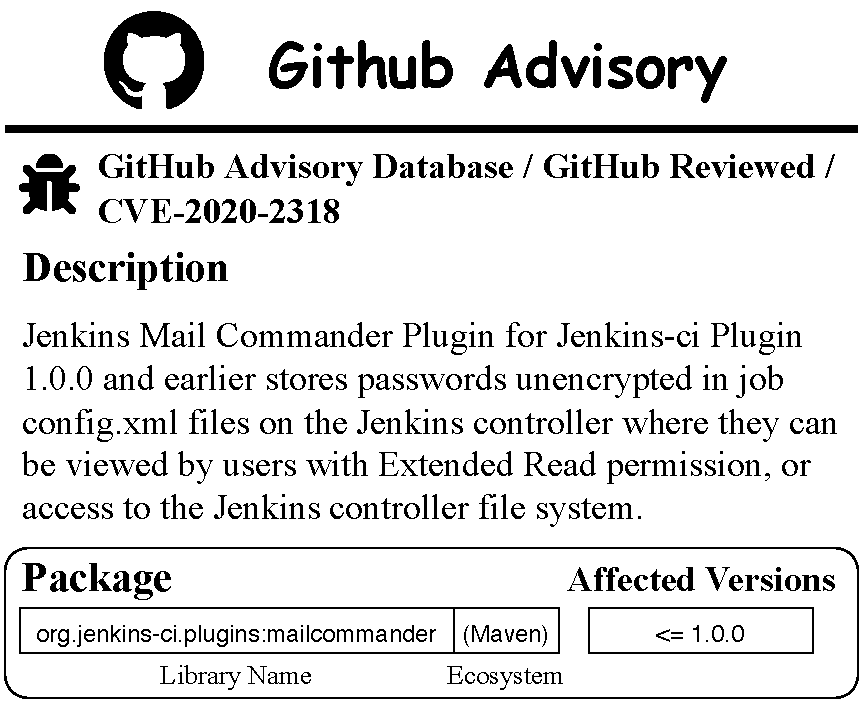
\includegraphics[width=1\linewidth]{figures/vulnerability-report.drawio.pdf}
\caption{GitHub Advisory Report for \href{https://github.com/advisories/GHSA-485q-v457-3p58}{CVE-2020-2318}}
\label{fig: case}
\vspace{-0.4cm}
\end{figure}

\section{Introduction}
\label{sec:intro}

One important task in security is to automatically extract the package names and versions affected by each security vulnerability. 
% With the increasing usage of third-party software packages, their security vulnerabilities pose great challenges to software and network systems.
A recent study~\cite{wang2020empirical} shows that 84\% third-party packages contain security vulnerabilities and 60\% of them are high-risk ones.
To mitigate the security risks, security practitioners maintain databases (e.g., NVD and GitHub Advisory) for each unique vulnerability (i.e., Common Weakness Enumeration or CVE). These databases contain reports with the vulnerability description, affected packages, and affected versions. For example, Figure~\ref{fig: case} shows the report of \href{https://github.com/advisories/GHSA-485q-v457-3p58}{CVE-2020-2318}. By linking the CVEs to the affected packages, developers can be aware of the vulnerable packages in their code and quickly apply patches/fixes; the affected packages also help with security knowledge management and task prioritization. Although developers can manually enter the affected packages when submitting CVEs, the entered information is often missing or incorrect~\cite{lightxml,viem}. While database maintainers also conduct manual reviews~\cite{githubReview}, automatic identification can accelerate the vulnerability lifecycle and reduce the manual costs, thus it is a critical task. 
%Figure~\ref{fig: case} shows an example report of one vulnerability, \href{https://github.com/advisories/GHSA-485q-v457-3p58}{CVE-2020-2318}.
%The vulnerability's affected packages include  \CodeIn{org.jenkins-ci.plugins:mailcommander} and its corresponding versions.
%The field of affected packages is specified by the developers who create this CVE. However, recent studies~\cite{lightxml,viem} show that in more than half of vulnerability reports, this field is missing or incorrect.
% \xueqing{can we say the package information is incorrect?}
% \tianyu{I think it's better not to mention incorrect, otherwise, our ground truth of labels might be challenged.}
%To alleviate this problem, human maintainers manually complete or validate the affected-package information in databases such as GitHub Advisory~\cite{githubReview}.
% \xueqing{replace reference inproceedings with misc}.
% \xueqing{Add citation to show that NVD or GitHub advisory packages are verified}.
%However, manual completion or validation requires high manual efforts~\cite{lightxml,vullibminer}, underscoring the need for automatic identification. 

% \xueqing{Explain how is smaller model used -> low accuracy -> leverage LLM's potential, LLM will keep improving-> if we use it the same way as smaller models, cost is high -> to leverage LLM wo high cost, propose the generative approach}

Several existing works have studied automatic affected package identification~\cite{fastxml, viem, lightxml, chronos, vullibminer}, however, it is challenging for them to achieve high accuracy because they fail to leverage large language models. Existing works typically rank/retrieve the package name from a list of pre-defined packages by computing the similarity between the vulnerability description and the package description. Since the time complexity of retrieval is linear to the size of the list (e.g., 435k Java packages), the cost of each model inference has to be kept quite low and only smaller models have been used, e.g., BERT and linear regression~\cite{fastxml,chronos,lightxml,vullibminer}. 

To leverage the extensive knowledge and semantic capabilities of LLMs, we propose a different strategy: \emph{generate rather than retrieve} the affected package. Our framework, \detector{}, is the first framework to directly generate the mentioned package name given the vulnerability description. Since generation requires the LLM inference to be invoked only once, our approach can easily scale to larger language models such as Llama-13B and Vicuna-13B on a single GPU server. 

% suffers from two related limitations on time cost and accuracy, respectively.  %lower accuracies while requiring a linear time cost with respect to the number of packages~\cite{chronos,vullibminer}. 
% First, existing work has linear time cost to the number of packages under consideration (e.g., 435k Java packages)~\cite{chronos,vullibminer}, so that the cost of each model inference has to be kept quite low. 
% Given a vulnerability description (Figure~\ref{fig: case}), existing work computes a similarity score between the vulnerability description and each package's text description from the ecosystem (e.g., PyPI, Maven), and then ranks all packages based on this score. As a result, the time cost for identifying each vulnerability = the number of candidate packages $\times$ the cost of each model inference (e.g., BERT). 
% Second, existing work suffers from low accuracy due to the adoption of a relatively small model. The first limitation causes the underlying model used for inference to be a relatively small model such as logistic regression and BERT~\cite{fastxml,chronos,lightxml,vullibminer}. 
% Second, regarding the time cost, given a vulnerability description (Figure~\ref{fig: case}), existing work requires to compute a similarity score between the vulnerability description and each package's text description from the ecosystem (e.g., PyPI, Maven), then they rank all package based on this score. As a result, the time cost for identifying each vulnerability = the number of candidate packages $\times$ the cost of each model inference (e.g., BERT). 

% To address the preceding limitations, in this paper, we propose the first work, a framework named \detector{}, to explore the use of a large language model (LLM) for identifying vulnerable packages, given the continuously and rapidly improved effectiveness brought by an LLM for various tasks. \detector{} uses an LLM to \emph{generate} the names of affected packages instead of ranking the names of packages under consideration. 
% Our rationale for not following the existing work's ranking approaches is that the number (denoted as $|\mathcal{P}|$) of packages under consideration (e.g., 435k Java packages) brings high cost to rank the similarity scores between a vulnerability and each package under consideration.
% In contrast, in order to identify vulnerable packages, the generative approach invokes the model inference only once, instead of $|\mathcal{P}|$ times.
% When using LLMs, we cannot directly adopt previous work's ranking approach, since the number of candidate packages (e.g., Java has 435k packages) and the inference cost of LLMs are both high. In contrast, the generative approach invokes the model inference only once.

%Specifically, \detector{} includes two techniques to address two main challenges of generating the names of affected packages.
Upon observing errors in the raw generation result of LLMs, we propose the following techniques for improving \detector{}'s accuracy. 
First, we conduct supervised fine-tuning (SFT), in-context learning, and retrieval-augmented generation (RAG) to enhance the domain knowledge of a LLM.
%as an LLM may lack the domain knowledge required to generate the name of the target package. During model inference, the vulnerability description as input fed to an LLM often does not contain the full information of the target package's name, and thus the LLM is required to infer the missing information based on  the domain knowledge. 
Second, we propose a novel local search technique to post-process the raw output for reducing hallucination, i.e., ensuring that the generated package name actually exists. Our local search algorithm is inspired by an empirical study of the incorrect raw outputs of ChatGPT. The study shows that most errors are partially correct, therefore we can create rules to match the incorrect part to the closest existing one given the correct part. Since the sub-level package information (e.g., \CodeIn{mailcommander} in Figure~\ref{fig: case}) is often more directly mentioned than the top-level package information (e.g., \CodeIn{org.jenkins-ci.plugins}), our local search algorithm first matches the suffix before the prefix. 

%Recent studies~\cite{vazquez2023javascript} show that an LLM may generate package names that do not exist. 
%Based on our empirical study of incorrect raw outputs of ChatGPT, we design our local search technique that matches the generation output with the closest package name among the names of the packages under consideration, and produces the matched package name as the final output.

% Second, to ensure the generated package exists, we propose a post-processing algorithm to match the generation output with the closest existing package name. Our algorithm design is based on an empirical study of the errors of the raw output of ChatGPT. 


% To address the preceding challenges, \detector{} includes two techniques. First, to enhance the domain knowledge of LLMs, we employ supervised fine-tuning, in-context learning, and retrieval-augmented generation (RAG). Second, to ensure the generated package exists, we propose a post-processing algorithm to match the generation output with the closest existing package name. Our algorithm design is based on an empirical study of the errors of the raw output of ChatGPT. 

% To improve the accuracy of the generation, \detector{} aims to address two issues with the generative approach. First, the LLM may lack the domain knowledge required to generate the target package. The reason is that the LLM's input vulnerability description often does not contain the full information of the package name, it thus requires the LLM to infer the missing information from the domain knowledge. Second, a previous study shows that the LLM may generate package names that do not exist. 

% To address the preceding issues, our approach includes two techniques. First, to enhance the domain knowledge of LLMs, we employ supervised fine-tuning, in-context learning, and retrieval-augmented generation (RAG). Second, to ensure the generated package exists, we propose a post-processing algorithm to match the generation output with the closest existing package name. Our algorithm design is based on an empirical study of the errors of the raw output of ChatGPT. 

% Existing work on automatic identification of vulnerable packages~\cite{fastxml, viem, lightxml, chronos, vullibminer} propose  ranking approaches\footnote{\xueqing{classification which can be seen as ranking approach}} that,  given the vulnerability description as the query, rank the most similar package name from an existing list of package names of the corresponding ecosystem (e.g., PyPI, Maven). Since a ranking approach requires one to compute the description's similarity with each package, the time cost is typically large, e.g., Java has 435k packages. To the best of our knowledge, most existing approaches focus on relatively smaller models such as non-neural-network models~\cite{fastxml}, logistic regression~\cite{zestxml,chronos}, or BERT~\cite{lightxml,vullibminer}. Without leveraging larger models, they typically suffer from low accuracies. 


% However, these approaches face the scalability problem due to the large number of third-party packages (e.g., more than 500 thousand).
% Now that it is time-consuming to correlate each package with a given vulnerability description, a large portion of existing approaches use only lightweight models, such as FastXML~\cite{fastxml} and ZestXML~\cite{chronos} to rank these packages, thus leading to low accuracies.
% Although other approaches~\cite{vullibminer} adopt reranking models after the lightweight ranking model, the number of candidate packages (e.g., 512) still leads to a heavy burden of time and computation resources, especially when adopting large language models (LLMs).

% Specifically, both of these approaches are limited to their training set~\cite{fernandez2011semantically}.
% Thus, they are ineffective in identifying unseen vulnerable libraries during training.

% To address the low accuracy issue, in this paper, we propose to first leverage large language models (i.e., 7B models and larger) for vulnerable package identification. Given the description, our approach will \emph{generate}, rather than rank the package names. As a result, our approach can scale to larger models since this approach requires invoking the model inference only once. However, it is unclear whether the generative approach is effective for this task. On the one hand, the description often does not include the full information about the package name (Section~\ref{sec: empirical_study}); on the other hand, the task requires the generated package name to exactly match the ground truth and previous work finds this to be challenging for LLMs~\cite{liu2023codegen4libs}. To understand the potential of the generative approach, we conduct a pilot study on the errors made by ChatGPT raw output for this task. The study shows that ChatGPT raw output has a reasonable accuracy; however, for some vulnerabilities, ChatGPT lacks the domain knowledge for generation; for other vulnerabilities, the generated package names do not exist. 
%Based on the study results,
% \xueqing{I named the task vulnerable package identification, please check}.
% Nevertheless, text generation suffers from challenges such as hallucination~\cite{ji2023survey} which may affect the accuracy. To understand the feasibility of the generative approach, we first conduct a pilot study on how ChatGPT output for this task. We observe that with 42\% probability, the raw output correctly matches the ground truth. Among the incorrect outputs, 22.4\% can be fixed by matching the output with the closest existing package.
% \xueqing{Check if this statement is true}.
%(3) Among the rest incorrect names, ChatGPT captures incorrect keywords or fails to capture keywords from vulnerability descriptions due to its lack of knowledge.
% From the results of the preceding empirical study, we categorize two main challenges that lead to incorrectly generated names.
% First, LLMs lack sufficient domain knowledge of these affected libraries.
% For example, a Java package's name consists of both group IDs and artifact IDs while the group ID might be neglected in a vulnerability description.
% Therefore, LLMs need to generate the correct group ID based on their domain knowledge.
% Second, LLMs might output non-existing package names.
% Note that LLMs generate the names of affected packages from only vulnerability descriptions, so the output names might have more/fewer tokens, e.g., \CodeIn{core} or \CodeIn{framework}, which are widely used in the names of Java packages.



% To address the preceding challenges, we design three techniques to address the preceding challenges.
% First, we design a retrieval augmented generation (RAG) technique that provides domain knowledge into the inputs of LLMs before generation.
% Specifically, we add the names of affected libraries generated by IR approaches as they might be similar to the targeted library names.
% Second, we design a constrained decoding algorithm during generation.
% We collect package names from ecosystems of each programming language and require the output of LLMs to include at least one of them, thus avoiding non-existing package names.
% This technique modifies the decoding layer of LLMs and can be applied to only open-source LLMs.
% Third, we design a local search algorithm after generation.
% It directly searches the closest package name for each generated name, thus also avoiding non-existing package names.
% This technique is non-intrinsic and can be applied to both commercial and open-source LLMs.


We evaluate \detector{} on four vulnerability ecosystems: Java, JS, Python and Go. Our evaluation attains three main findings. First, we observe that the accuracy of \detector{} (0.806) significantly outperforms existing ranking approaches using smaller models~\cite{fastxml,lightxml,chronos,vullibminer} (0.721) and the computational time costs are comparable. 
%In particular, \detector{} using Vicuna-13B outperforms the larger ChatGPT and GPT-4 models by employing supervised fine-tuning (SFT). 
Second, our ablation studies show that SFT, RAG, and local search all help improve the accuracy of \detector{} and SFT contributes to the most improvement. In particular, the fine-tuned open-source Vicuna-13B outperforms the unfine-tuned commercial ChatGPT and GPT-4 models. Our local search algorithm can significantly reduce the hallucination in the original LLM output, and it is especially helpful for longer package names such as Java and Go. Third, \detector{} provides high value to security practice: at the time of the writing, we have submitted 60 pairs of <vulnerability, affected package> to GitHub Advisory (25 Java, 14 JS, 11 Python, 10 Go) and 34 of them have been accepted and merged.
% Additionally, the source code and dataset of \detector{} can be found in \url{https://github.com/q5438722/VulLibGen}.
% To examine \detector{}'s performance in the real-world setting, we further randomly sample a subset of the vulnerability descriptions in Java and JS, use \detector{} to generate the package names, and submit the generated names to GitHub Advisory. Among the 28 submitted <vulnerability, affected package> pairs, 22 are accepted and merged. This result highlights the real-world performance of \detector{} in automatically generating the names of affected packages. 

% We evaluate \detector{} using four state-of-the-art/practice (SOTA) approaches (FastXML~\cite{fastxml}, LightXML~\cite{lightxml}, Chronos~\cite{chronos}, and VulLibMiner~\cite{vullibminer}) that identify vulnerable libraries on the dataset of GitHub Advisory.
% Our evaluation results show that:
% (1) \detector{} is highly effective, achieving an accuracy of 0.806 while the best of SOTA approaches achieves only 0.669.
% (2) Our RAG technique and local search algorithm can boost the effectiveness of \detector{} by 8.9\% and 3.0\% on average, respectively.
% (3) \detector{} achieves better trade-offs between efficiency and accuracy than both existing and future ranking approaches.
% (4) \detector{} brings high value to security practice. 
% We have submitted 28 pairs of <vulnerability, affected package> to GitHub advisory, and 22 of them have been accepted and merged.
% We submit 25 vulnerabilities' affected libraries to GitHub advisory and 18 of them are accepted and merged.
% (5) Although fine-tuned open-source LLMs achieve similar effectiveness with ChatGPT/GPT4, they might face the limitation of overfitting, which can be alleviated by larger open-source LLMs.\tianyu{is it necessary to keep (5)?}



% Existing approaches~\cite{fastxml, viem, lightxml, chronos, vullibminer} model this task as an information retrieval (IR) task or a classification task.
% For example, they take the description field \CodeIn{``Jenkins Mail Commander Plugin for Jenkins-ci Plugin 1.0.0 and earlier stores passwords unencryted $\dots$''} as inputs and their targeted outputs, are the field of affected libraries, e.g., \CodeIn{maven:org.jenkins-ci.plugins:mailcommander}.
% However, these approaches face the scalability problem as it is unavoidable for IR/classification approaches.
% Specifically, both of these approaches are limited to their training set~\cite{fernandez2011semantically}.
% Thus, they are ineffective in identifying unseen vulnerable libraries during training.

% To address the scalability problem, in this paper, we propose to model this task as a generation task, thus utilizing the tremendous capabilities of Large Language Models (LLMs) in comprehending vulnerability descriptions.
% Here, we collect the dataset from the reviewed reports in GitHub Advisory.
% The affected libraries in each report are submitted by library developers and users, and they are manually validated by the maintainers of GitHub Advisory.
% Therefore, the ground truth of this dataset is reliable.
% Specifically, the number of Java, JavaScript, Python, and Go vulnerabilities are 4308, 3193, 2237, and 1351, respectively.


% Before employing LLMs for this task, we conduct an empirical study on the results when directly querying ChatGPT, revealing two main categories of challenges faced by LLMs.
% First, LLMs lack sufficient domain knowledge of these affected libraries.
% For example, in CVE-2022-24197, the affected library is \CodeIn{maven:com.itextpdf:itext7-core} while its description only mentions the affected library's artifact ID \CodeIn{itext7-core}, and its group ID \CodeIn{com.itextpdf} is neglected. 
% This group ID can be complemented based on the domain knowledge that only \CodeIn{itext7-core} corresponds to only one group ID \CodeIn{com.itextpdf}.
% Second, LLMs might output non-existing library names.
% For example, in CVE-2020-2167, the affected library is \CodeIn{maven:com.openshift.jenkins:openshift-pipeline} while LLMs might change the group ID into \CodeIn{com.openshift.jenkins}, which is not an existing library.
% % \tianyu{I also consider the reason that there might exist vulnerabilities whose descriptions are incomplete. (in the following comments in the source code)
% % However, this reason might be similar to 'lack of domain knowledge'}
% % First, the information in vulnerability reports might be incomplete. 
% % For example, in CVE-2017-1000406, the affected library is \CodeIn{maven:org.opendaylight.integration:distribution-karaf} while token \CodeIn{distribution} does not occur in its description.
% % Thus, even human experts cannot identify the correct names of affected libraries.


% To address the preceding challenges, we design two categories of techniques to address the preceding challenges.
% First, we design a retrieval augmented generation (RAG) technique that provides domain knowledge into the inputs of LLMs. 
% Specifically, we add the names of affected libraries generated by IR approaches as they might be similar to the targeted library names.
% Second, we design a constrained decoding algorithm and a local search algorithm to reduce non-existing outputs.
% Specifically, the constrained decoding algorithm is more effective while the local search algorithm is non-intrinsic and can be applied in commercial LLMs, e.g., ChatGPT/GPT4.
% Both algorithms utilize the database of all library names (e.g., those in Maven or Pypi) to ensure that the output of \detector{} is an existing library name.


% We evaluate \detector{} using three state-of-the-art/practice (SOTA) approaches (LightXML~\cite{lightxml}, Chronos~\cite{chronos}, and VulLibMiner~\cite{vullibminer}) that identify vulnerable libraries on the dataset of GitHub Advisory.
% Our evaluation results show that:
% (1) \detector{} is highly effective, achieving an accuracy of 0.80 while the best of SOTA approaches achieves only 0.669.
% (2) Our RAG technique can boost the effectiveness of both ChatGPT/GPT4 and open-source LLMs by at least 12\%.
% (3) Both our constrained decoding and local search algorithms can effectively reduce incorrect/non-existing outputs by at least 5.4\%.
% (4) \detector{} brings high value to security practice. We submit 25 vulnerabilities' affected libraries to GitHub advisory and 18 of them are accepted and merged.
% (5) Although fine-tuned open-source LLMs achieve similar effectiveness with ChatGPT/GPT4, they might face the limitation of overfitting, which can be alleviated by larger open-source LLMs.


% 一个建议的intro提纲:
% 1. CVE问题的重要性(为什么需要自动预测,可以帮助及时修补?)
% 2.当前解决方案的不足(scalability)
% 3.我们提出用generation来解决scalability问题,介绍一下GitHub advisory数据集以及为什么ground truth是准确的,3.但是generation存在挑战:一个是有的example input信息不全(所以即使human expert也很难做到100%),一个是llm缺乏domain knowledge 
% 4.做一个empirical study发现input信息不全的现象只占少数。同时针对以上挑战,设计了几个方法:fine tuning,rag,constrained decoding,post processing,讨论一下它们为什么有可能解决generation的挑战。
% 5. 总结实验结果,讨论可能存在的limitation,比如fine tuning可能存在overfitting,future work如何弥补这些limitation


% To avoid potential risks posed by vulnerabilities in third-party libraries, security researchers maintain databases containing vulnerability reports, e.g., the National Vulnerability Database (NVD)~\cite{nvd}. 
% A vulnerability report in NVD includes a vulnerability's identification number in the entry of Common Vulnerability Enumeration (CVE), its description, and the name list of libraries affected by the vulnerability  (a.k.a. vulnerable libraries).
% Application developers can identify vulnerable libraries by directly querying each description and CPE entry with the name of each used library. 
% However, recent studies on about 200,000 vulnerability reports in NVD show that 53.3\% of the vulnerability reports in NVD do not mention any affected libraries~\cite{lightxml} and 59.82\% of the included vulnerable libraries are incomplete or incorrect~\cite{viem}.


% To address the preceding issue, existing approaches~\cite{viem, anwar2021cleaning, jo2022vulcan, kuehn2021ovana, fastxml, lightxml, chronos, vullibminer} fall into three main categories.
% First, named-entity-recognition (NER) approaches~\cite{viem, anwar2021cleaning, jo2022vulcan, kuehn2021ovana} use NER models to extract the mentioned library entities from vulnerability descriptions, and then match these entities with a dictionary of library names.
% Second, extreme multi-label learning (XML) approaches~\cite{fastxml, lightxml, chronos} use deep-learning classification models to assign a set of labels (i.e., vulnerable libraries) to a given vulnerability by training on labeled datasets.
% Third, entity-linking approaches~\cite{vullibminer} take library descriptions as inputs besides the description of a given vulnerability, thus achieving higher accuracy than NER and XML approaches.

% Although existing approaches make efforts to identify vulnerable libraries, they still suffer from highly inaccurate results.
% Existing NER and XML approaches cannot distinguish vulnerable libraries with similar names, such as ``org.jenkins-ci.plugins:mailer'' and ``org.jenkins-ci.plugins:mailcommander''.
% However, these libraries are not affected together by one vulnerability due to their different functionalities and scopes.
% Existing entity-linking approaches use TF-IDF techniques to reduce the number of libraries for comparison, and yet suffer from false negatives (i.e., some vulnerable libraries are missed) and thus low accuracy.
% Considering the large number of collected libraries (e.g., 310,844 in Maven) for comparison compared, this step cannot be avoided; otherwise, it might cost them two years to identify all vulnerable libraries~\cite{vullibminer}.




% To overcome the preceding limitations, we propose \detector{}, the first generative approach to generate the affected libraries of a given vulnerability.
% \detector{} is effective to generate the name list of vulnerable libraries (out of all the existing libraries) by utilizing the recent enormous advances in Large Language Models (LLMs) with two stages of fine-tuning.
% The rationale behind this step is that LLMs can correlate the input vulnerability description to vulnerable libraries based on their prior knowledge of these libraries, e.g., their functionalities, usages, and even history issues.
% With prior knowledge, \detector{} avoids the high cost of correlating one vulnerability description with each library.
% Specifically, we conduct unsupervised fine-tuning on maven~\cite{maven} corpus to fine-tune raw LLaMa models to activate their prior knowledge of Java libraries.
% The input of this stage is one library's description, and its targeted output is its library name.
% Then, we conduct supervised fine-tuning on labeled datasets to enhance the ability to identify vulnerable libraries.
% The input of this stage is a vulnerability description and its targeted output is a name list of vulnerable libraries affected by this vulnerability.

% Since we use fine-tuned LLMs to generate the affected library names of a given vulnerability, there are two main challenges that decrease LLMs' effectiveness.
% First, LLMs face the difficulty of low accuracy when identifying zero-shot libraries because they have no prior knowledge of how these libraries are affected by vulnerabilities.
% Similar to XML approaches, LLMs tend to output incorrect libraries that have already been affected by other vulnerabilities during training and fine-tuning.
% Second, LLMs face hallucinations, i.e., generating plausible-looking library names that are non-existing.
% For example, they might mix up two similar library names and lack part of the library names.



% To address the preceding challenges, we design two specialized techniques during supervised fine-tuning to improve the effectiveness by addressing the preceding challenges.
% To help identify zero-shot libraries, we design an input augmentation technique, which feeds the names of vulnerable libraries (a.k.a., recommended libraries) identified by the SOTA approach~\cite{vullibminer} to \detector{} as input.
% This technique provides examples of libraries whose functionalities are likely to be affected by a given vulnerability.
% Thus, \detector{} can generate library names from those with similar functionalities instead of all libraries when \detector{} has no prior knowledge of how these zero-shot libraries are affected by vulnerabilities.
% To address \detector{}'s hallucinations, we design our post-processing technique based on the Levenshtein distance~\cite{levenshtein} to obtain existing Java library names from the response of LLMs.
% We find that \detector{} can generate the components of the targeted library names (i.e., the targeted functionalities and scopes), and make mistakes when jointing these components of library names, thus leading to hallucinations.
% Therefore, hallucination library names are close to the targeted names of vulnerable libraries, and their closest library names tend to be the targeted names.


% We evaluate \detector{} using three state-of-the-art/practice approaches (LightXML~\cite{lightxml}, Chronos~\cite{chronos}, and VulLibMiner~\cite{vullibminer}) that identify vulnerable libraries on an open-source dataset (VulLib)~\cite{vullib}.
% Our evaluation results show a number of findings to demonstrate our \detector{} approach’s effectiveness and efficiency.
% Given the ground truth score of 0.840, \detector{} effectively achieves the F1@1 score of 0.626 while the state-of-the-art/practice (SOTA) approaches achieve only 0.561.
% Specifically, the post-processing technique helps \detector{} achieve an average improvement of F1@1 by 9.3\%, and the input augmentation technique helps \detector{} achieve an average improvement of F1@1 by 39\% in identifying zero-shot libraries.
% Additionally, \detector{} is highly efficient, identifying one vulnerability in less than 6 seconds.


% In summary, this paper makes the following main contributions:
% \begin{itemize}
% \item  We propose, \detector{}, the first generative approach for identifying vulnerable libraries via Large Language Models.
% \item  We design an input augmentation technique and a post-processing technique to help identify zero-shot libraries and help address hallucinations.
% \item  We conduct a comprehensive evaluation demonstrating the effectiveness and efficiency of \detector{}, increasing the F1@1 of 0.626 while the state-of-the-art/practice (SOTA) approaches achieve only 0.561.
% \end{itemize}


%\section{Problem Overview}\label{sec: background}
%formalize the task of identifying vulnerable libraries and introduce the scalability limitation of existing ranking approaches.
% To address the scalability limitation, we model this task as a generation task based on the results of an empirical study and then investigate the challenges of generating the names of affected packages.


\begin{table*}[t]
    \centering
    \caption{An Empirical Study on ChatGPT's Incorrect Response in Maven (Java ecosystem)}
    \label{tab: fault case study}
\scriptsize
\begin{threeparttable}
\begin{tabular}{p{2cm}p{1.8cm}p{4.3cm}p{4.3cm}}
\toprule
\textbf{Error Reason}                                            & Example (w/ link)                             & ChatGPT's Output                                                   & Ground Truth (Affected Packages)                                                         \\
\midrule
\multirow{2}{*}{\makecell[l]{\textbf{Type 1: Incorrect}\\ \textbf{but exist (23\% of}\\ \textbf{ all errors)}}} & \href{https://github.com/advisories/GHSA-9qhq-j4xm-cw48}{CVE-2015-3158}                     & org.\textcolor{Blue}{picketlink:picketlink}                                    & org.\textcolor{Blue}{picketlink:picketlink-tomcat}-common                                     \\
&&  \multicolumn{2}{l}{\textit{Description:} ``The invokeNextValve function in \textit{identity/federation/bindings/\textcolor{Blue}{tomcat}/idp/AbstractIDPValve.java}}                             \\
&& \multicolumn{2}{l}{in \textcolor{Blue}{PicketLink} before 2.7.1.Final does not properly check role based authorization, which allows remote} \\
&& \multicolumn{2}{l}{authenticated users to gain access to restricted application resources via a (1) direct request $\dots$'' } \\
\midrule
\multirow{8}{*}{\makecell[l]{\textbf{Type 2: Non-Exist,}\\ \textbf{Partially correct}\\ \textbf{(58\% of all errors)}}}                                          & \href{https://github.com/advisories/GHSA-wv88-pf73-x22p}{CVE-2011-2730}                     & org.\textcolor{Blue}{springframework}:\textcolor{Red}{spring-framework}                                    & org.\textcolor{Blue}{springframework}:\textcolor{Blue}{spring-core}                                      \\
&&  \multicolumn{2}{l}{\textit{Description:} ``VMware \textcolor{Blue}{SpringSource Spring Framework} before 2.5.6.SEC03, 2.5.7.SR023, and 3.x before  }                                                                                                                                                                                \\
&& \multicolumn{2}{l}{ 3.0.6, when a container supports Expression Language (EL), evaluates EL expressions in tags twice which } \\
& & \multicolumn{2}{l}{allows remote attackers to obtain sensitive information. $\dots$''}                                                                                                                                                                                \\
\cmidrule(lr){3-4}
% , and ChatGPT mistakes token ``\textcolor{BrickRed}{framework}'' in its artifact ID.
  & \href{https://github.com/advisories/GHSA-264w-xrr7-6qqg}{CVE-2020-2167}                       & \textcolor{Red}{org.jenkins-ci.plugins}:\textcolor{Blue}{openshift-pipeline}                    & \textcolor{Blue}{com.openshift.jenkins}:\textcolor{Blue}{openshift-pipeline}                       \\
&&\multicolumn{2}{l}{\textit{Description:} ``\textcolor{Blue}{OpenShift Pipeline Plugin} 1.0.56 and earlier does not configure its YAML parser to prevent} \\
&&\multicolumn{2}{l}{
the instantiation of arbitrary types. This results in a remote code execution (RCE) vulnerability exploitable}                                                                                                                                                                      \\
&& \multicolumn{2}{l}{  by users able to provide YAML input files to OpenShift Pipeline Plugin’s build step. $\dots$''}                                                                                                                                                                      \\
 % without the group id, so ChatGPT uses a widely used one ``\textcolor{BrickRed}{org.jenkins-ci.plugins}''.
\midrule
% \textbf{More/Fewer Tokens}                      & 28                        & \href{https://github.com/advisories/GHSA-3v63-f83x-37x4}{CVE-2015-1830}                       & org.apache.activemq:activemq                                 & org.apache.activemq:activemq-client                            \\
% \multicolumn{5}{l}{\textit{Description:} ``Directory traversal vulnerability $\dots$ in \textcolor{ForestGreen}{Apache ActiveMQ} 5.x before 5.11.2 $\dots$'', and ChatGPT lacks the token ``\textcolor{ForestGreen}{client}''.}                                                                                                                                                                                      \\
% \midrule
\multirow{4}{*}{\makecell[l]{\textbf{Type 3: Non-Exist,}\\ \textbf{Completely incorrect}\\ \textbf{(19\% of all errors)}}}&                      \href{https://github.com/advisories/GHSA-jpj4-5xwp-cv23}{CVE-2020-11974}                      & \textcolor{Red}{mysql:mysql-connector-java}                                   & \textcolor{Blue}{org.apache.dolphinscheduler:dolphinscheduler}                   \\
&& \multicolumn{2}{l}{\textit{Description:} ``In \textcolor{Blue}{DolphinScheduler} 1.2.0 and 1.2.1, with \textcolor{Red}{mysql connector} a remote code execution vulnerab}\\
&& \multicolumn{2}{l}{-ility
exists when choosing mysql as database.''}                          \\
\cmidrule(lr){3-4}
% , and ChatGPT incorrectly captures ``\textcolor{BrickRed}{mysql}''.
&          \href{https://github.com/advisories/GHSA-fxp8-7h5w-h235}{CVE-2019-13234}                      & \textcolor{Red}{N/A}                                                                  & \textcolor{Blue}{org.opencms:opencms-core}                                       \\
&&\multicolumn{2}{l}{\textit{Description:} ``In the Alkacon \textcolor{Blue}{OpenCms} Apollo Template 10.5.4 and 10.5.5 there is XSS in the search engine.''}  \\
% , and ChatGPT repeats the unstructured description.
\bottomrule
\end{tabular}
% \begin{tablenotes}
%     \item A Java package name consists of two parts, [group id]:[artifact id]
% \end{tablenotes}
\end{threeparttable}
\vspace{-0.3cm}
\end{table*}



%\subsection{Task Formalization}~\label{sec: formal}
%\noindent \textbf{Target:}


% and the developer description may not explicitly differentiate between them\xueqing{provide a concrete example}. 

%The following is backup
% Given a natural language description of the vulnerability associated with a software package (e.g., Figure~\ref{fig: case}), the goal is to identify the software package that the description refers to. For example, the description in Figure~\ref{fig: case} refers to the Java package \CodeIn{org.jenkins-ci.plugins:mailcommander}. The referred package must be within the existing packages of the ecosystem (e.g., Table~\ref{tab: dataset info}). The ground truth package name is verified by expert maintainers from the GitHub advisory database~\cite{githubReview}. From Figure~\ref{fig: case} we observe that the identification of the package name is a non-trivial problem that goes beyond token-level matching. The challenges of this NLP task lie in the following folds: first, a part of the target package name is missing in the description, which requires domain knowledge for bridging this gap\xueqing{provide a concrete example}; second, some package names are similar, so it is easy to confuse between them, e.g., \CodeIn{org.jenkins-ci.plugins} and \CodeIn{io.jenkins.plugins} are two most common group IDs in Java, and the developer description may not explicitly differentiate between them\xueqing{provide a concrete example}. 


%The mapping results are defined as subsets of $\mathcal{L}$ as one vulnerability can affect more than one package: $\forall v \in \mathcal{V}, \mathcal{F}(v) \subseteq \mathcal{L}$.

% \noindent \textbf{Labelled Dataset:}

% The dataset $\mathcal{D}$ of this task includes $(\mathcal{V_D}, \mathcal{L_D}, \mathcal{F_D})$ where $\mathcal{V_D}$ is a set of collected vulnerabilities, $\mathcal{F_D}$ is the labels (affected packages) of these vulnerabilities, and $\mathcal{L_D}$ is naturally defined as $\mathcal{F_D}(V_D)$.

% The target of existing approaches is to learn the correlation from a given dataset $\mathcal{F^{'}} \sim \mathcal{F_D}$.



\section{Existing Work on Vulnerable Package Identification\label{sec: scale}}

This section summarizes existing work on affected package identification and analyze the scalability challenge. 

\noindent \textbf{Formal Definition of Affected Package Identification}. Given a security vulnerability (CVE) submitted to a software ecosystem (e.g., GitHub Advisory), the goal of affected package identification is to link the description $q$ of the CVE to an existing software package name $p$ (e.g., a Maven or PyPi package) that is affected by the CVE. An example of the linked package can be found in Figure~\ref{fig: case}, where the description mentions the affected package \CodeIn{org.jenkins-ci.plugins:mailcommander}. 

%select one or more affected packages $p$ from a list $\mathcal{P}$ of existing packages of an ecosystem. 

\noindent \textbf{Smaller Models Have Lower Accuracies}. 
%At test time, existing work computes the similarity score $sim(p, q)$ for each $p\in\mathcal{P}$, where $p$ is represented by its description documentation in the ecosystem. As a result, the time cost on each vulnerability = $|\mathcal{P}| \times$ the cost to compute each similarity score. 
Existing approaches on vulnerable package identification~\cite{fastxml, viem, lightxml, chronos} all suffer from lower accuracies~\cite{chronos,vullibminer}. Given the vulnerability $q$, existing works rank all packages $p$ of the ecosystem by computing the similarity score between the descriptions of $q$ and $p$. Due to the large number of packages (e.g., Maven has 435k packages), existing work cannot afford using large language model to compute the score. All of them thus rely on smaller models, e.g., logistic regression~\cite{zestxml,chronos} and BERT~\cite{lightxml,vullibminer}. Despite various methods introduced for improving the accuracy~\cite{viem, anwar2021cleaning}, the accuracies remain low~\cite{vullibminer}.

\noindent \textbf{Existing Work's Efforts on Scaling to Larger Models}. To improve the accuracy, existing work leverages re-ranking with the BERT model~\cite{vullibminer}. More specifically, they first use TF-IDF to rank all packages in the ecosystem (435k in Java and 506k in Python), then re-rank the top-512 packages using BERT. The re-ranking approach achieves a reasonable accuracy with a saved inference cost, but there remains a large room for improving the accuracy~\cite{vullibminer}.

%While the recall@512 of TF-IDF is 0.9, their Accuracy@1 is far from 0.9. 

%For example, by treating each candidate package as a class and performing extreme multilabel classification~\cite{fastxml,lightxml}, or using language models to rank the candidate packages~\cite{vullibminer}. 
% In the ranking problem, the computational cost is large due to the large number of candidate packages (435k in Java and 506k in Python). Existing ranking approaches typically rely on more efficient smaller models such as non-neural networks or logistic regression~\cite{zestxml,chronos}.
% and BERT~\cite{lightxml,vullibminer}. 
%In particular, the inference time for a 13B LLM (440M model) for each vulnerability is approximately 200 hours (20 mins) on an A100 GPU.
% \tianyu{10 mins already use ranking +reranking, otherwise, it might cost more than 200 hours}. 
% Due to the limitation in the model size, existing work often suffers from low accuracies~\cite{chronos, vullibminer}. 

%\noindent\textbf{Using Re-Ranking to Scale Up}. To leverage the potential of larger models, existing work adopts a re-ranking approach~\cite{vullibminer}.
% \xueqing{Check if there exists other reranking approach}. \tianyu{Fudan has one accepted ICSE'24 paper, Holmes, which has not been published yet, so I think it's proper not to mention it.}
%Given the vulnerability description, this approach first uses TF-IDF to rank all packages (e.g., 435k in Java), then re-ranks the top-512 packages using a 440M BERT model, the time cost for the re-ranking approach is approximately $512\times 2 milliseconds = 1 second$. Although they argue that TF-IDF has a recall@512 of 0.9, their final performance still has a large gap compared to this number. While re-ranking can also leverage larger models, it requires a much higher time cost: for example, for a 13B LLM, the time cost is approximately 20 mins on one A100 GPU.
% \xueqing{check this}

 % \xueqing{rephrase}

% \noindent\textbf{\xueqing{Using Vector Database to Scale Up}}. 
% \tianyu{It is not a standard vector, it needs to map the package name to vulnerability descriptions}


\section{Two Challenges with LLM Generation~\label{sec: empirical_study}}

%to investigate the potential of LLM -> cannot adopt ranking -> generation. However generation has 2 challenges. 

In contrast to existing work, we propose the first work, \detector{}, that leverages LLMs for affected package identification. Due to the scalability challenge of the retrieval approach, our approach directly \emph{generates rather than retrieves} the affected package. \detector{} thus only need to invoke the LLM inference once for each vulnerability $q$.  
% Formally speaking, given the vulnerability description $q$, the generative approach directly generates the affected package names $p$, therefore the time cost on each vulnerability = $1\times$the inference cost of the LLM. 
Nevertheless, there exist two challenges with the generative approach. 

\noindent \textbf{Challenge 1: Lack of Domain Knowledge}. The first challenge is that there may exist a knowledge gap for the LLM to generate the correct package. This is because the description may not contain the full information about the affected package name. For example, \href{https://github.com/advisories/GHSA-264w-xrr7-6qqg}{CVE-2020-2167} in Table~\ref{tab: fault case study} is about the Java package \CodeIn{com.openshift.jenkins.openshift-pipeline}, but the the description does not mention the word "\emph{Jenkins}". To predict the correct package name, the LLM has to rely on domain knowledge to complete this information. Existing work have used various methods to bridge the knowledge gap of LLMs, e.g., supervised fine-tuning~\cite{prottasha2022transfer, church2021emerging} and retrieval augmented generation~\cite{lewis2020retrieval,
mao2020generation, liu2020retrieval, cai2022recent}. 


\noindent \textbf{Challenge 2: Generating Non-Existing Package Names}. Following a previous study on Reddit\footnote{\url{https://www.reddit.com/r/ChatGPT/comments/zneqyp/chatgpt\_hallucinates\_a\_software\_library\_that/}}, the second challenge is that the LLM may generate library names that do not exist in the ecosystem. Existing work has adopted post-processing to reduce the non-existing package issue in code translation and program repair~\cite{jin2023inferfix, roziere2021leveraging}. Following existing work, we can potentially leverage post-processing by matching the generated package with the closest existing package.  %based on their edit distance. 

To understand whether post-processing is promising for solving Challenge 2 and to study how to design the post-processing algorithm, we conduct an empirical study on ChatGPT's incorrect response, the study result can be seen in Table~\ref{tab: fault case study}. The study uses 2,789 Java vulnerability descriptions collected in a recent work~\cite{vullibminer}. We divide all ChatGPT responses into four types: 1. the package is incorrect but it exists (13\%, 23\% of errors); 2. the package does not exist and is partially correct (34\%, 58\% of errors); 3. the package is completely incorrect (11\%, 19\% of errors). 4. the package is correct (42\% of all cases); 

\begin{figure*}[t]
\centering
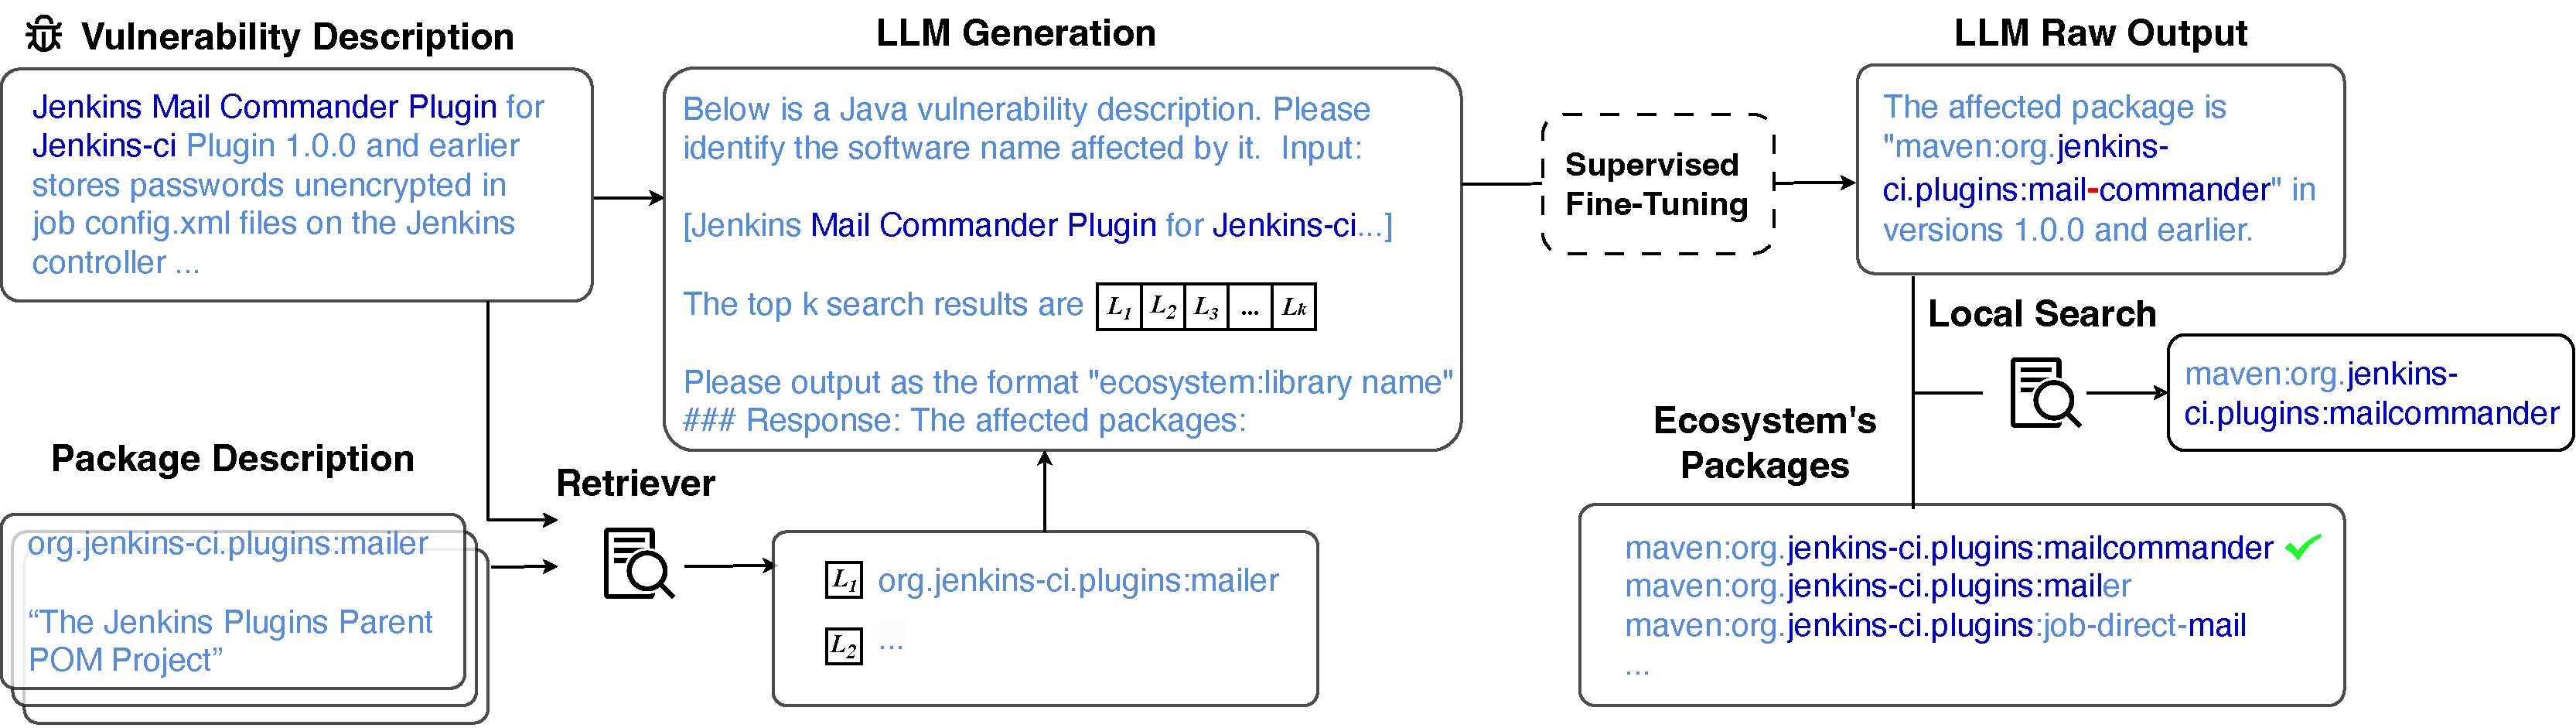
\includegraphics[width=1\linewidth]{figures/workflow-v3.drawio.pdf}
\caption{The \detector{} Framework}
\label{fig: framework}
\vspace{-0.3cm}
\end{figure*}

From the study result, we draw the conclusion that post-processing by matching is a promising approach to solve Challenge 2. This is because the majority errors are Type 2 errors, while post-processing is the most effective in helping with Type 2 errors. For example, for \href{https://github.com/advisories/GHSA-264w-xrr7-6qqg}{CVE-2020-2167}, ChatGPT generates \textcolor{Red}{org.jenkins-ci.plugins}:\textcolor{Blue}{openshift-pipeline}. While the \textcolor{Blue}{suffix} is correct, the \textcolor{Red}{prefix} and \textcolor{Blue}{suffix} never co-occur in any existing package name. We can fix this case by matching the prefix to the closest co-occured one. 
%The average edit distance between ChatGPT output and the ground truth in Type 2 cases is 76\%. 
By applying a naive edit-distance matching on the ChatGPT output, the accuracy is improved from 42\% to 51\%. 



%We start by querying ChatGPT with 2,789 Java vulnerability descriptions collected in a recent work~\cite{vullibminer}. ChatGPT outputs the correct package names (exactly matching) 42\% of the time. Next, we randomly sample 100 from the remaining incorrect ones and manually annotate the error reasons. Since all Java packages are in the format of [group id]:[artifact id], we classify the errors into the 4 classes in Table~\ref{tab: fault case study}. First, for the first two types (63\%), either the group ID or the artifact ID is correct, we thus further try matching the generation output with the closest package name (based on edit distance), and find that 34.9\% errors can be fixed. For example, the generation output for \href{https://github.com/advisories/GHSA-264w-xrr7-6qqg}{CVE-2020-2167} contains the group id \CodeIn{com.openshift.jenkins} which does not exist. On the other hand, the closest package in the existing list is the correct one. Second, for the last two types of errors there exists a knowledge gap for ChatGPT to identify the correct package name.

%, e.g., ChatGPT fails to identify that DolphinScheduler refers to the package \CodeIn{org.apache.dolphinscheduler}. 
%From the pilot study result we conclude that: while the generative approach has a reasonable baseline accuracy, there exists room for potential improvement by matching the generation output with existing package names and enhancing the knowledge of the LLM. 


% \begin{table*}[t]
%     \centering
%     \caption{The Classified Reasons for ChatGPT's Incorrect Response in Maven}
%     \label{tab: fault case study}
% \scriptsize
% \begin{tabular}{lclll}
% \toprule
% \textbf{Fault Reason}                         & Number                    & Example                             & ChatGPT's Output                                                   & Ground Truth (Affected Packages)                                                         \\
% \midrule
% \textbf{Mixed Artifact ID}                    & 21                        & \href{https://github.com/advisories/GHSA-wv88-pf73-x22p}{CVE-2011-2730}                     & org.springframework:spring-framework                                    & org.springframework:spring-core                                      \\
% \multicolumn{5}{l}{\textit{Description:} ``VMware \textcolor{ForestGreen}{SpringSource Spring Framework} before 2.5.6.SEC03, $\dots$'', and ChatGPT mistakes token ``\textcolor{BrickRed}{framework}'' in its artifact ID.}                                                                                                                                                                                \\
% \midrule
% \textbf{Mixed Group ID}                       & 15                        & \href{https://github.com/advisories/GHSA-264w-xrr7-6qqg}{CVE-2020-2167}                       & org.jenkins-ci.plugins:openshift-pipeline                    & com.openshift.jenkins:openshift-pipeline                       \\
% \multicolumn{5}{l}{\textit{Description:} ``\textcolor{ForestGreen}{OpenShift Pipeline} Plugin 1.0.56 and earlier $\dots$'' without the group id, so ChatGPT uses a widely used one ``\textcolor{BrickRed}{org.jenkins-ci.plugins}''.}                                                                                                                                                                      \\
% \midrule
% \textbf{More/Fewer Tokens}                      & 28                        & \href{https://github.com/advisories/GHSA-3v63-f83x-37x4}{CVE-2015-1830}                       & org.apache.activemq:activemq                                 & org.apache.activemq:activemq-client                            \\
% \multicolumn{5}{l}{\textit{Description:} ``Directory traversal vulnerability $\dots$ in \textcolor{ForestGreen}{Apache ActiveMQ} 5.x before 5.11.2 $\dots$'', and ChatGPT lacks the token ``\textcolor{ForestGreen}{client}''.}                                                                                                                                                                                      \\
% \midrule
% \textbf{Misleaded Name}                       & 23                        & \href{https://github.com/advisories/GHSA-jpj4-5xwp-cv23}{CVE-2020-11974}                      & mysql:mysql-connector-java                                   & org.apache.dolphinscheduler:dolphinscheduler                   \\
% \multicolumn{5}{l}{\textit{Description:} ``In \textcolor{ForestGreen}{DolphinScheduler} 1.2.0 and 1.2.1, with \textcolor{BrickRed}{mysql} connector $\dots$'', and ChatGPT incorrectly captures ``\textcolor{BrickRed}{mysql}''.}                          \\
% \midrule
% \textbf{No Structural Output}                            & 13                        & \href{https://github.com/advisories/GHSA-fxp8-7h5w-h235}{CVE-2019-13234}                      & -                                                                  & org.opencms:opencms-core                                       \\
% \multicolumn{5}{l}{\textit{Description:} ``In the Alkacon \textcolor{ForestGreen}{OpenCms} Apollo Template 10.5.4 and 10.5.5 $dots$'', and ChatGPT repeats the unstructured description.}  \\
% \bottomrule
% \end{tabular}
% \end{table*}



% \noindent \textbf{A Generation Task:}

% \subsection{Challenges of Adopting LLMs}~\label{sec:empirical_study}

% Before employing LLMs to generate the names of affected libraries, we conduct an empirical study to investigate the challenges when directly querying LLMs.







% \subsubsection{Lack Sufficient Domain Knowledge}
% First, LLMs lack sufficient domain knowledge of these affected libraries.
% For example, in CVE-2022-24197, the affected library is \CodeIn{com.itextpdf:itext7-core} while its description only mentions the affected library's artifact ID \CodeIn{itext7-core}, and its group ID \CodeIn{com.itextpdf} is neglected. 
% This group ID can be complemented based on the domain knowledge that only \CodeIn{itext7-core} corresponds to only one group ID \CodeIn{com.itextpdf}.
% Second, LLMs might output incorrect (even non-existing) library names.



% \subsection{Our Motivation}


% \noindent \textbf{Model Inference:} For a set of unlabeled vulnerabilities $\mathcal{V}_{new}$, we use one learned mapping relationship, $\mathcal{M^{\prime}}$, to predict these vulnerabilities' affected libraries, $\mathcal{M^{\prime}} (\mathcal{V}_{new})$, which is a subset of all libraries $\mathcal{L}$.


% \subsection{Existing Approaches of Identifying Vulnerable Libraries}

% \textbf{LightXML:} LightXML~\cite{lightxml} is one representative XML approaches that identify vulnerable libraries. 
% It takes the input of a vulnerability's description and outputs the order of a set of candidate libraries.
% Specifically, LightXML represents vulnerability descriptions based on transformer-based models, e.g., BERT~\cite{bert} or RoBERTa~\cite{roberta}.
% Then it uses generative cooperative networks to score all label clusters divided by a balanced K-means~\cite{da2008structural} algorithm.
% In a recent study~\cite{lightxml}, LightXML is more effective and efficient than its preceding approaches, such as ExtremeText~\cite{wydmuch2018no}, Bonsai~\cite{khandagale2020bonsai} and FastXML~\cite{fastxml}.
% Now that LightXML takes only the library names as labels, it can only predict full-shot libraries, i.e., $\mathcal{L}_{train}$.


% \textbf{Chronos:} Chronos~\cite{chronos} is another representative XML approach.
% Similar to other XML approaches, it also takes the input of a vulnerability's description and outputs the order of a set of candidate libraries.
% Chronos represents vulnerability descriptions and library names by TF-IDF and uses one SOTA XML algorithm, ZestXML to determine possible vulnerable libraries.
% Although ZestXML can identify vulnerable libraries from a candidate library set with a little portion of zero-shot ones, e.g., $\mathcal{L}_{train} \cup \mathcal{L}_{test}$ (2,817 libraries)~\cite{chronos}, it also fails to identify zero-shot libraries from all Java libraries, $\mathcal{L}$ (310,844 libraries).


% \textbf{VulLibMiner:} VulLibMiner~\cite{vullibminer} is one representative entity-linking approach that identifies vulnerable libraries. 
% It takes the descriptions of a vulnerability and all libraries as inputs.
% VulLibMiner first uses a TF-IDF algorithm to filter out a subset of candidate libraries and uses a BERT-FNN network on each pair of <vulnerability, candidate library> to determine whether they are correlated.
% A recent study~\cite{vullibminer} shows that VulLibMiner is more effective than XML approaches, especially in identifying zero-shot libraries.
% Considering the large number of Java libraries (e.g., 310,844 in Maven) for comparison compared, the TF-IDF algorithm cannot be avoided, and yet causes false negatives (i.e., some vulnerable libraries are missed).


% \subsection{Large Pre-trained Language Models}
% Large Pre-trained Language Models (LLMs) mainly follow the Transformer~\cite{vaswani2017attention} structure with an encoder to encode a given input and a decoder to generate output sequences from the encoded representation.
% These LLMs include billions of parameters and are pre-trained on billions of language corpus on the internet.
% In recent years, LLMs, such as GPT-3/4~\cite{gpt3, openai2023gpt4}, LLaMa~\cite{llama}, and starcoder~\cite{starcoder}, have been widely applied in software engineering~\cite{chen2021evaluating, xia2022practical} and security~\cite{chan2023transformer, tony2023llmseceval} tasks.
% Additionally, LLMs can comprehend the descriptions of vulnerabilities, thus improving the effectiveness of downstream tasks, such as vulnerability type classification~\cite{liu2023not} and providing attack and defense guidance~\cite{abdeen2023smet}.


% Although LLMs perform well in comprehending vulnerability descriptions, they face the hallucination challenge~\cite{maynez2020faithfulness, shuster2021retrieval}, where LLMs generate plausible-looking results that are factually incorrect. 
% Specifically, they might mix up two similar entities (e.g., library names), or make errors where just one token is incorrect.
% A recent study~\cite{lee2023benefits} shows that even one of the largest LLM, GPT-4~\cite{openai2023gpt4} cannot avoid hallucinations.
% Considering the large number of Java library names, addressing hallucinations becomes one of the main challenges of identifying vulnerable libraries.

%
% \noindent \textbf{Zero-shot Library Identification:} The affected libraries of $\mathcal{V}_{new}$ might not occur in the training dataset due to the data imbalance of the large number of Java libraries (310,844) and the small number of affected Java libraries (2,811 and 985 in two recent work~\cite{fastxml, vullibminer}).
% Therefore, the model is required to identify unseen libraries during prediction, and this task is established in machine learning as zero-shot learning~\cite{wang2019survey}.

% If denote $\mathcal{L}_{train}$ and $\mathcal{L}_{test}$ as the vulnerable library sets of the training and testing set, zero-shot libraries are defined as libraries not occurred in the training set:
% \begin{equation}
%     \mathcal{L}_{zero} = \{l \in \mathcal{L}_{test} \mid l \not\in \mathcal{L}_{train}\} 
% \end{equation}

% Then, zero-shot vulnerabilities are vulnerabilities affecting only zero-shot libraries.
% We divide the testing set, $\mathcal{V}_{test}$, into two independent subsets, zero-shot vulnerabilities, $\mathcal{V}_{zero}$, and non-zero-shot (a.k.a, full-shot) vulnerabilities, $\mathcal{V}_{full}$. 
% \begin{equation}
%     \begin{aligned}
%         \mathcal{V}_{zero} &= \{ v \in \mathcal{V}_{test} \mid \mathcal{M} (v) \subseteq \mathcal{L}_{zero} \} \\
%         \mathcal{V}_{full} &= \{ v \in \mathcal{V}_{test} \mid \mathcal{M} (v) \not\subseteq \mathcal{L}_{zero} \} \\
%     \end{aligned}
% \end{equation}

% These two subsets can be used to evaluate the effectiveness of identifying zero-shot vulnerable libraries and full-shot ones.



% \xueqing{tick color is green; make the red dash more obvious}  

\section{\detector{} Framework}\label{sec:approach}

To address the two challenges in LLM generation, we employ the following techniques: first, we use supervised fine-tuning and in-context learning to enhance the domain knowledge in LLM; second, we further employ the retrieval-augmented framework (RAG) to enhance the knowledge when SFT is not easy; third, we design a local search technique which alleviates the non-existing package name problem. The \detector{} framework can be found in Figure~\ref{fig: framework} \footnote{Our prompt in Figure~\ref{fig: framework} is: "\emph{Below is a [Programming Language] vulnerability description. Please identify the software name affected by it. Input: [DESCRIPTION]. The top k search results are: [$L_1$][$L_2$]$\cdots$[$L_k$]. Please output the package name in the format "ecosystem:library name".
\#\#\# Response: The affected packages:}". ~\label{fn: input}}.
% \tianyu{using the same input/output format for both fine-tuning and inference}

\subsection{Supervised Fine-Tuning/In-Context Learning}

To solve the first challenge (Section~\ref{sec: empirical_study}), we incorporate supervised fine-tuning~\cite{prottasha2022transfer, church2021emerging} and in-context learning~\cite{dong2022survey, olsson2022context} in \detector{}. For SFT, we use the full training data (Table~\ref{tab: dataset info}); for ICL, we randomly sample 3 examples from the training data for each evaluation vulnerability. For both SFT and ICL, the input and output of the LLM follow the following format: Input: the same prompt as Figure~\ref{fig: framework}~\footref{fn: input}, Output: "\emph{The affected package is [package name]}". The hyper-parameters used for ICL and SFT are listed in Table~\ref{tab: hyper parameter} of Appendix.
% \xueqing{The 3 examples can be seen in Table...of appendix}
% \xueqing{confirm random sampling?} 
% ""\xueqing{fill input}

% \xueqing{For SFT, explain the input/output training data, hyperparameters (appendix), and the fact that we train different models for different PLs }

\subsection{Retrieval-Augmented Generation (RAG)}

%Retrieval augmented generation (RAG) is a framework that enhances the performance of a generative model by injecting the top-k most relevant search result in the prompt~\cite{lewis2020retrieval,gao2023retrieval}. 
To further enhance the LLM's domain knowledge especially when SFT is not easy (e.g., ChatGPT and GPT4), we employ retrieval-augmented generation (RAG) in \detector{}.

\noindent \textbf{Retriever Setting}. Given the description of a vulnerability, our retriever ranks existing package names in an ecosystem (Table~\ref{tab: dataset info}) based on the similarity score between the vulnerability description and the package description. The descriptions of Java, JavaScript, Python, and Go packages are obtained from Maven~\footnote{\url{https://mvnrepository.com}}, NPM~\footnote{\url{https://www.npmjs.com}}, Pypi~\footnote{\url{https://pypi.org}}, and Go~\footnote{\url{https://pkg.go.dev}} documentations.
For example, the description of the package \CodeIn{org.jenkins-ci.plugins:mailcommander} is \textit{``This plug-in provides function that read a mail subject as a CLI Command.''}.
Our retriever follows \cite{vullibminer}'s re-ranking strategy, i.e., first rank all packages (e.g., 435k in Java) using TF-IDF, then re-rank the top 512 packages using a BERT-base model fine-tuned on the same training data in Table~\ref{tab: dataset info}.
% \xueqing{check}

% \xueqing{check consistency with introduction: BERT only vs BERT and TF-IDF}.
% \tianyu{we follow the similar idea of VulLibMiner, use TF-IDF + BERT to retrieve xxx}
% \tianyu{maybe bert-only is ok as the reranking step do not consider TF-IDF}


\subsection{Local Search}

To solve the second challenge (Section~\ref{sec: empirical_study}), we incorporate post-processing in \detector{}.
Based on the empirical study results in Section~\ref{sec: empirical_study}, we design a local search technique to match the generation output with the closest package name from an existing package list (Algorithm~\ref{alg: local search} in Appendix~\ref{sec: local search algorithm}). 

Algorithm~\ref{alg: local search} employs the edit distance as the metric and respects the structure of the package name. Formally, a package name can be divided into two parts: its prefix and suffix (separated by a special character, e.g., `:' in Java).
The prefix (e.g., the artifact ID of Java packages) specifies the maintainer/group of this package, and the suffix (e.g., the group ID of Java packages) specifies the functionalities of this package.
Specifically, Java, Go, and part of JS packages can be explicitly divided while Python and the rest of JS packages only specify their functionalities in their names.
We denote the prefix of a package name as empty if it can not be divided.

Algorithm~\ref{alg: local search} first compares the generated suffix with all existing suffix names and matches the suffix to the closest one. After fixing the suffix, we can then obtain the list of prefixes that co-occur at least once with this suffix. We match the generated prefix with the closest prefix in this list.
The reason that we opt to match the suffix first is twofold. First, our study shows that the vulnerability description more frequently mentions the suffix than the prefix: among all 2,789 vulnerabilities investigated in Section~\ref{sec: empirical_study}, their description mentions 12.4\% of the tokens in the prefixes of the affected packages and 66.0\% of the tokens in their suffixes of the affected packages;
% Specifically, the vulnerability description mentions 12.4\% of the tokens of the prefixes and 66.0\% of the suffixes;
% \tianyu{more explanations}
second, our study also shows that each suffix co-occurs with fewer unique prefixes than conversely.
In all 435k Java packages, each prefix has 5.86 co-occurred suffixes while each suffix has only 1.13 co-occurred prefixes on average.
As a result, it is easier to identify the prefix by first matching the suffix, and then matching the suffix with the co-occurred prefix list. 
% \xueqing{Fix here}
% \xueqing{add study of the frequency to Section 3}
% \xueqing{add study of the frequency to Section 3}

%there exist more suffix package names (e.g., 200k in Java) than prefix package names (e.g., 20k in Java).  
% For example, there are more than 200,000 unique suffixes in the Maven ecosystem and less than 20,000 unique prefixes.
% Therefore, fixing the suffix first reduces LLMs' generation capability less than fixing the prefix first.
% \tianyu{let me consider why}
% \tianyu{correlates to using grammar to reduce syntactical errors, maybe replacing 'local search' with another name}


% Additionally, we conduct a two-staged local search when given a Java vulnerability because the names of Java packages are relatively complex and structural compared to package names of other programming languages. 
% A Java package name consists of its group ID and artifact ID.
% In this scenario, we first search for an existing artifact ID and then search for an existing group ID corresponding to this artifact ID.
% Our rationale is that the artifact IDs include each package's functionalities, which is easier to identify from a vulnerability's description.


% \subsection{During Generation: Constrained Decoding}

% We design our constrained decoding algorithm to restrict the open-source LLMs to include the name of at least one existing package.
% This constraint is written as follows:

% \begin{equation*}
%     \exists l \in \mathcal{L}, \mbox{ s.t. } l \in \mathcal{F}_{generation} (v)
% \end{equation*}

% However, adopting constrained decoding has two technical challenges to address.
% First, each package name contains more than one token (e.g., Python packages have 6 tokens on average) while LLMs generate only one token at once.
% Therefore, we cannot greedily check whether the constraints are satisfied during decoding.
% To address this challenge, we construct a Trie tree to represent the constraints (as shown in Figure~\ref{fig: framework}) and then conduct beam search~\cite{kumar2013beam} to ensure that the output contains at least one path (corresponding to an existing package name) on this Trie tree.

% Second, the large number of packages in each ecosystem (e.g., 435,642 in Maven and 506,848 in Pypi) brings a heavy efficiency burden as the Trie tree for constrained decoding might have more than 1,000,000 nodes. 
% We empirically notice that invoking an LLM with 7B parameters might cost more than 2 hours, which is unacceptable.
% To address this challenge, we relax the ``hard'' constraints to ``soft'' ones.

% Our implementation of ``soft'' constraints consists of two steps.
% (1) We replace the entire Trie tree with a bi-gram Trie tree with only two depth of nodes.
% For example, if a package name consists of three tokens \CodeIn{[``org'', ``google'', ``gson'']}, we add two edges in this bi-gram Trie tree, \CodeIn{``org''} $\rightarrow$ \CodeIn{``google''} and \CodeIn{``google''} $\rightarrow$ \CodeIn{``gson''}.
% The bi-gram Trie tree can remove a large portion (more than 50\%) of leaf nodes in the Trie tree, thus substantially speeding up beam searching during decoding.
% (2) We add another term of probability $\log p_{trie} (w_{i+1}|w_{i})$ to ensure that the output is quite similar to an existing package name.
% Specifically, when decoding the i+1 th token $w_{i+1}$, each token's probability $p(w_{i+1}|w_{0:i})$ is defined as follows:
% \begin{equation*}
%     \begin{aligned}
%         \log p(w_{i+1}|w_{0:i}) \propto &\lambda_{LLM} \log p_{LLM}(w_{i+1}|w_{0:i})\\
%         + &\lambda_{cons} \log p_{trie} (w_{i+1}|w_{i})\\
%         p_{trie}(w_{i+1}|w_{i}) \propto &\ \sum_{l \in \mathcal{L}, j} l[j,j+1] = w[i,i+1]
%     \end{aligned}
% \end{equation*}
% where $\lambda_{LLM}$ and $\lambda_{cons}$ are two hyper-parameters that determine the respective contribution of an LLM and our constraints. 

% \tianyu{is it necessary to mention trie tree with top512 results?}

% % To address this challenge, we follow the similar idea of VulLibMiner, using a TF-IDF~\cite{jones1972statistical, jones2004idf} technique to filter a small candidate of packages.
% % Its empirical results indicate that 512 is a proper candidate size with a recall of at least 0.9.
% % Thus, the decoding constraint is modified as:

% % \begin{equation*}
% % \begin{aligned}
% %     &\mathcal{L}(v) = \mathop{\mbox{Top512}}\limits_{l_i \in \mathcal{L}}\ TF\mathit{-}IDF(v, l_i) \\
% %     &\exists l \in \mathcal{L}(v), \mbox{ s.t. } l \in \mathcal{F}_{generation} (v)
% % \end{aligned}
% % \end{equation*}

% % However, this resolution




% Unlike conventional information retrieval (IR)/classification approaches, \detector{} utilizes the tremendous capabilities of Large Language Models (LLMs) in comprehending vulnerability descriptions.
% Our key insight is that conventional approaches highly depend on their training set and thus face the scalability problem and this problem can be alleviated by modeling this task as a generation task.

% As formalized in Section~\ref{sec: formal}, the training input of \detector{} includes the textual descriptions of vulnerabilities, $\mathcal{V}$, the textual descriptions of all Java libraries in Maven, $\mathcal{L}$, and the mapping relationship from vulnerabilities to libraries, $\mathcal{M}$.
% When applied in practice, \detector{} takes only the textual descriptions of one vulnerability as input and outputs a series of names of libraries affected by this vulnerability.


% \begin{figure}[t]
% \centering
% 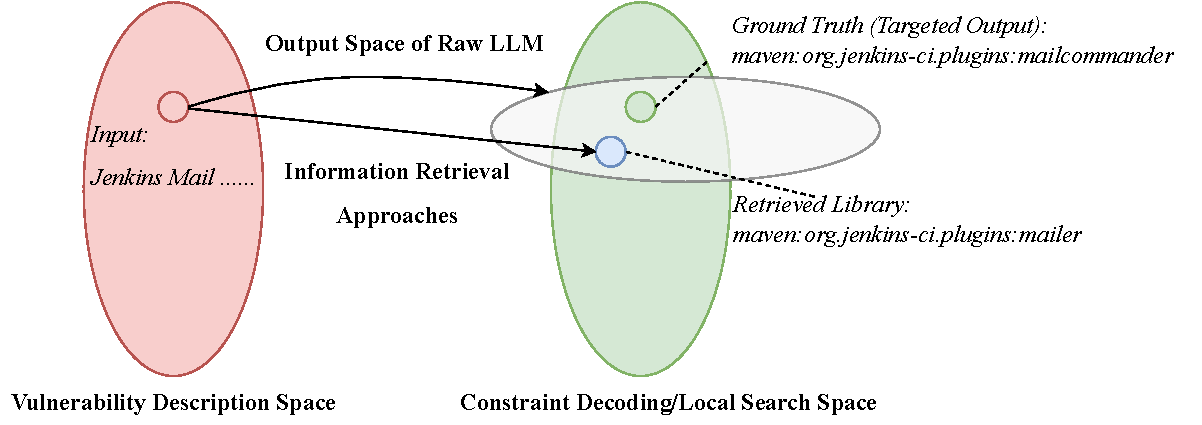
\includegraphics[width=1\linewidth]{figures/approach-illustration.drawio.pdf}
% \caption{An Illustration of the Motivation of our RAG and Constrained Decoding/Local Search Techniques}
% \label{fig: case}
% \end{figure}

% \subsection{Fine-tuning and Prompt-tuning}




% LLMs can correlate the input vulnerability description to vulnerable libraries based on their prior knowledge of these libraries, e.g., their functionalities, usages, and even history issues.

% As formalized in Section~\ref{sec: formal}, the training input of \detector{} includes the textual descriptions of vulnerabilities, $\mathcal{V}$, the textual descriptions of all Java libraries in Maven, $\mathcal{L}$, and the mapping relationship from vulnerabilities to libraries, $\mathcal{M}$.
% When applied in practice, \detector{} takes only the textual descriptions of one vulnerability as input and outputs a series of names of libraries affected by this vulnerability.


% The process of \detector{} is shown in Figure~\ref{fig: framework} with two steps.
% First, we conduct unsupervised fine-tuning on Maven Corpus, which includes all Java libraries and their descriptions.
% This step aims at activating their knowledge of each Java library, including its name and functionalities.
% Second, we conduct supervised fine-tuning on the input dataset $(\mathcal{V}, \mathcal{L}, \mathcal{M})$ to learn the mapping relationship from vulnerabilities to libraries.



% During supervised fine-tuning, we design two specific techniques to improve the effectiveness of \detector{}.
% To help identify zero-shot libraries, we design an input augmentation technique, which feeds the names of vulnerable libraries (a.k.a., recommended libraries) identified by the SOTA approach~\cite{vullibminer} to \detector{} as input.
% This technique provides examples of libraries whose functionalities are likely to be affected by a given vulnerability.
% Thus, \detector{} can generate library names from those with similar functionalities instead of all libraries when \detector{} has no prior knowledge of how these zero-shot libraries are affected by vulnerabilities.
% To address \detector{}'s hallucinations, we design our post-processing technique based on the Levenshtein distance~\cite{levenshtein} to obtain existing Java library names from the response of LLMs.
% We find that \detector{} can generate the components of the targeted library names (i.e., the targeted functionalities and scopes), and make mistakes when jointing these components of library names, thus leading to hallucinations.
% Therefore, hallucination library names are close to the targeted names of vulnerable libraries, and their closest library names tend to be the targeted names.


% \subsection{Two Stages of Fine-Tuning with Input Augmentation}
% \detector{} mainly consists of two stages of fine-tuning on LLMs.
% In this paper, we choose one of the state-of-the-art (SOTA) open-source LLMs, LLaMa~\cite{llama}, as our base LLM with 7B and 13B parameters.

% During unsupervised fine-tuning, \detector{} takes the input of one library description, and its targeted output is its library name.
% Table~\ref{tab: lib-aws} shows an example case in this step.
% Its input describes the functionality of this package, e.g., configuration on AWS plugins, and its output is a structural Java library name, \CodeIn{maven:io.jenkins.plugins: aws-global-configuration}.
% The rationale of unsupervised fine-tuning is to activate their knowledge of each Java library by correlating each Java library's functionality description with its name. 

% After unsupervised fine-tuning, \detector{} conducts supervised fine-tuning on the input dataset, $(\mathcal{V}, \mathcal{L}, \mathcal{M})$ with two steps.
% First, \detector{} invokes another approach of identifying vulnerable libraries to recommend a list of vulnerable library names for input augmentation.
% Note that our rationale for input augmentation is to help identify zero-shot libraries because LLMs have no prior knowledge of how these libraries are affected, so we choose two representative approaches that effectively identify zero-shot libraries.
% Specifically, we choose VulLibMiner and the TF-IDF matcher in VulLibMiner because each of them identifies zero-shot and full-shot (non-zero-shot) libraries with a similar F1 score~\cite{vullibminer} while the TF-IDF matcher, as a NER approach, is less effective than VulLibMiner.
% Second, \detector{} concatenates the description of a given vulnerability with the recommended libraries as the input prompt used for supervised fine-tuning.
% The targeted output in this step is a name list of vulnerable libraries that are affected by this vulnerability.

% Table~\ref{tab: cve-mail} shows an example case of \CodeIn{CVE-2020-2318} in this step.
% The description of this vulnerability mentions the vulnerable functionality, \CodeIn{Jenkins Mail Commander Plugin}, its package source, \CodeIn{Jenkins-ci Plugin 1.0.0}, and how this vulnerability is exploited.
% We also show that the recommended library is another Java library with the same group id and a similar artifact id.
% However, \detector{} rejects this recommended result and outputs the correct vulnerable library, thus indicating its generation capability instead of simply judging whether recommended libraries are correct or not.







% \subsection{Post-Processing of Library Names}





% \begin{algorithm}[t]
% \caption{Post-Processing of Library Names}
% \label{alg: post-processing}
% \begin{algorithmic}[1]
% \Require $rawResponse$, raw text of LLM's Response.
% \Require $libMaven$, Java library names from Maven.
% \Ensure $vulnNames$, a list of vulnerable library names.
% \Function{Post-Processing}{$rawResponse, libMaven$}
%     \State $rawNames \gets rawResponse.findall(\mbox{``maven:\textbackslash 
%  w*:\textbackslash w*''})$
%     \State $artifacts \gets \emptyset{}, groups \gets \{ \}$
%     \For{$mavenName \in libMaven$}
%         \State $\mbox{``maven''}, groupid, artifactid \gets mavenName.split()$
%         \State $artifacts.append(artifactid)$
%         \State $groups[artifactid].append(groupid)$
%     \EndFor
%     \For{$rawName \in rawNames$}
%         \State $\mbox{``maven''}, groupid, artifactid \gets rawName.split()$
%         \State $Levenshtein.weight \gets (W_{insert}, W_{delete}, W_{replace})$
%         \State $artifactid^{\prime} \gets \mathop{argmin}\limits_{id \in artifacts}{Levenshtein(artifactid, id)}$
%         \State $subgroups \gets groups[artifactid^{\prime}]$
%         \State $groupid^{\prime} \gets \mathop{argmin}\limits_{id \in subgroups}{Levenshtein(groupid, id)}$
%         \State $vulnNames \gets \mbox{``maven''}: groupid^{\prime}: artifactid^{\prime}$
%     \EndFor
%     \State \Return{$vulnNames$}
% \EndFunction
% \end{algorithmic}
% \end{algorithm}

% To address \detector{}'s hallucinations, we design our post-processing technique based on the Levenshtein distance~\cite{levenshtein} to obtain existing Java library names from the response of LLMs.
% We find that \detector{} can generate the components of the targeted library names (i.e., the targeted functionalities and scopes), and make mistakes when jointing these components of library names, thus leading to hallucinations.
% Therefore, hallucination library names are close to the targeted names of vulnerable libraries, and their closest library names tend to be the targeted names.



% To address \detector{}'s hallucinations, we design our post-processing algorithm based on the Levenshtein distance~\cite{levenshtein} to obtain correct Java library names from the response of LLMs.
% Our goal is to ensure that the generated library names belong to existing Java libraries.
% One major difficulty for this problem is that Java library names are relatively complex and structural when compared with library names of other programming languages.
% A correct Java library name consists of its group id and artifact id.
% Here we take only libraries collected in Maven into consideration, so we add a prefix identifier, \CodeIn{maven}, before each library name.
% Thus, an example of correct Java library names is \CodeIn{maven:com.google.code.gson:gson}.

% Our post-processing algorithm is designed based on the rationale that hallucinations library names are slightly different from the real names of vulnerable libraries.
% For example, the group id of a Java library consists of multiple components separated by periods (\CodeIn{.}) and some of these components might be neglected or incorrectly replaced.
% Therefore, we use Levenshtein distance to find the correct affected libraries.

% Our technique is shown in Algorithm~\ref{alg: post-processing}.
% It takes the raw-text output of our fine-tuned LLM and outputs a list of vulnerable library names after post-processing.
% This algorithm conducts post-processing through two steps: parsing the raw-text output into a list of library names, and identifying their closest existing library names.

% In Line 2, we parse the raw-text output into a list of library names.
% Here we use a regex expression that contains the identifier ``maven'', group id, and artifact id, to extract library names from our fine-tuned LLM's output, $rawResponse$.

% In Lines 3-16, we identify the closest library names based on the library names extracted in the first step.
% In Lines 3-8, we divide the names of all Java libraries in Maven into multiple groups where library names in each group have the same artifact id.
% In Lines 9-10, for each generated library name, we first split it into its group id and artifact id.
% In Line 12, we use its artifact id, $artifactid$ to find its closest and existing artifact id, $artifactid^{\prime}$.
% Then in Lines 13-14, we use its group id, $groupid$ to find its closest and existing group id, $groupid^{\prime}$ from library names with the same artifact id, $artifactid^{\prime}$.
% Then, we concatenate the ``maven'' identifier with the search results, $groupid^{\prime}$ and $artifactid^{\prime}$ as one post-processed library name.
% Additionally, in Line 11, we manually set the weight used in calculating Levenshtein distances because LLMs change the library names in terms of tokens instead of characters.
% Thus, the weight of inserting one character should be smaller than that of deleting and replacing one, and we set the empirical Levenshtein weights as follows, $W_{insert} = 1, W_{delete} = 4, W_{replace} = 4$.
% \begin{equation}
%     W_{insert} = 1, W_{delete} = 4, W_{replace} = 4
% \end{equation}

% Our empirical statistics show that the average length of tokens in library names is 5.7, and their average number of different characters is 1.7



% \tianyu{group id reflect the sources of library, artifact id reflects its functionalities}

% \CodeIn{maven:com.sdklite:gson}
% Thus, library names generated by LLMs might neglect part of the components or include more components.


% \begin{table}[t]
% \renewcommand\arraystretch{1}
% \centering
% \caption{An Example of Java Library}
% \label{tab: lib-aws}
% \begin{tabular}{p{1.8cm}|p{6cm}}
% \toprule
% Input Prompt              & Below is a Java lib description \\
% \midrule
% \makecell[l]{Library\\ Description} & \makecell[l]{Input: Configure all AWS related plugins from\\ a single page.} \\
% \midrule
% \makecell[l]{Model\\ Response} & \makecell[l]{This package's name is\\ \textit{maven:io.jenkins.plugins:aws-global-configuration}.}\\
% \bottomrule
% \end{tabular}
% \end{table}


% \begin{table}[t]
% \centering
% \caption{An Example of CVE-2020-2318}
% \label{tab: cve-mail}
% \begin{tabular}{p{1.8cm}|p{6cm}}
% \toprule
% Input Prompt              & Below is a Java vulnerability description.   Please identify the software name affected by it \\
% \midrule
% Vulnerability Description & Input: Jenkins Mail Commander Plugin for Jenkins-ci Plugin 1.0.0 and   earlier stores passwords unencrypted in job config.xml files on the Jenkins   controller where they can be viewed by users with Extended Read permission,   or access to the Jenkins controller file system. \\
% \midrule
% \makecell[l]{Recommended\\ Library}       & \makecell[l]{Top 1 search result are \textit{maven:org.jenkins-ci.plugins:job-direct-mail}} \\
% \midrule
% \makecell[l]{Model\\ Response} & \makecell[l]{The affected packages is\\ \textit{maven:org.jenkins-ci.plugins:mail-commander.}}\\
% \midrule
% \makecell[l]{Post-processed\\ Library}    & \makecell[l]{\textit{maven:org.jenkins-ci.plugins:mailcommander}} \\
% \bottomrule
% \end{tabular}
% \end{table}
\section{Evaluation}
\label{sec:evalution}

\subsection{Evaluation Setup}

\noindent \textbf{Dataset}. Among existing work on affected package identification~\cite{fastxml,lightxml,chronos,vullibminer}, two datasets are frequently used: VeraCode~\cite{fastxml} and VulLib~\cite{vullibminer}. In this work, we choose to use VulLib instead of VeraCode because it is of better quality. The VulLib dataset contains 2,789 Java vulnerabilities collected from GitHub Advisory. Each package name in VulLib is manually verified by security experts from GitHub Advisory~\cite{githubAD}. In contrast, VeraCode is not verified thus it is prone to errors~\footnote{VeraCode does not use explicit package names ecosystems. For example, the affected package of CVE-2014-2059 is ``org.jenkins-ci.main:jenkins-core'' while VeraCode labels it as three packages: ``jenkins'', ``openshift-origin-cartridge-jenkins'', and ``jenkins-plugin-openshift''}.
% \xueqing{add footnote to explain}.
Since VulLib only focuses on Java, we further extend it to JS, Python and Go by collecting the data from GitHub Advisory following a similar workflow as VulLib. 


% In this paper, we evaluate the effectiveness of \detector{} using the GitHub Advisory database, since each vulnerability in GitHub Advisory is manually reviewed and verified by expert maintainers~\cite{githubReview}.
% In GitHub Advisory, the vulnerabilities are classified by the associated Programming languages~\cite{githubAD}, therefore we can construct a list of programming language-focused datasets~\footnote{Specifically, we extend VulLib, a Java dataset proposed by ~\cite{vullibminer} with the same workflow. 
% Our rationale is that with the help of security experts' verification, VulLib addresses the data quality limitation of VeraCode, another dataset proposed by ~\cite{fastxml} and used by FastXML, LightXML, and Chronos.}. 


% Existing ranking approaches (FastXML, LightXML, Chronos) focus on using the dataset collected by ~\cite{fastxml}, while the ground truths in that dataset are not verified and the quality is low. 
% To improve the data quality, ~\cite{vullibminer} proposed a new dataset VulLib, where the ground truths are verified by security experts of the GitHub advisory~\cite{githubReview}.
% However, VulLib is limited to Java.

% In this work, we extend VulLib to all four languages with the same workflow (thus the ground truths are all verified).
% Additionally, in GitHub Advisory, the vulnerabilities are classified by the associated Programming languages~\cite{githubAD}, therefore we can construct a list of programming language-focused datasets. 

% In this paper, we evaluate the effectiveness of \detector{} using the GitHub Advisory database, since each vulnerability in GitHub Advisory is manually reviewed and verified by expert maintainers~\cite{githubReview}. In GitHub Advisory, the vulnerabilities are classified by the associated Programming languages~\cite{githubAD}, therefore we can construct a list of programming language-focused datasets. 

%Our dataset focuses on four widely used programming languages: Java, JavaScript (JS), Python, and Go. 
The statistics of our dataset are listed in Table~\ref{tab: dataset info}. In total, our dataset includes 2,789 Java, 3,193 JS, 2,237 Python, and 1,351 Go vulnerabilities, respectively. To the best of our knowledge, this is the first dataset for identifying vulnerable packages with various programming languages. For each PL, we split the train/validation/test data with the 3:1:1 ratio. The split is in chronological order to simulate a more realistic scenario and to prevent lookahead bias~\cite{lookahead_bias}.

% Our dataset focuses on four widely used programming languages: Java\footnote{For Java, we use VulLib~\cite{vullibminer}, which is expanded from the Java vulnerabilities in GitHub Advisory.}, JavaScript (JS), Python, and Go. The statistics of our dataset are listed in Table~\ref{tab: dataset info}. In total, our dataset includes 2,789 Java, 3,193 JS, 2,237 Python, and 1,351 Go vulnerabilities, respectively. To the best of our knowledge, this is the first dataset for identifying vulnerable packages with various programming languages. For each PL, we split the train/validation/test data with the 3:1:1 ratio. The split is in chronological order to simulate a more realistic scenario and to prevent lookahead bias~\cite{lookahead_bias}.



%In this table, we also include the number of packages in each ecosystem and their average tokens, which both affected the difficulty of generating package names.
% This table shows that there are 45.41\% zero-shot packages (i.e., not affected by vulnerabilities in the training set), and 36.02\% zero-shot vulnerabilities (i.e., affect only zero-shot packages).
% As discussed in Section~\ref{sec: formal}, we divide the testing set, $\mathcal{L}_{test}$ into $\mathcal{L}_{zero}$, and $\mathcal{L}_{full}$, to evaluate the effectiveness of identifying zero-shot and full-shot vulnerable packages.

\begin{table}[t]
\centering
\caption{The Statistics of the GitHub Advisory Dataset}
\label{tab: dataset info}
\begin{threeparttable}
\small
\begin{tabular}{lrrrr}
\toprule
           & Java & JS   & Python & Go   \\
\midrule
\multicolumn{5}{l}{\textit{\#Vulnerabilities:}}     \\
Training   & 1,668 & 1,915 & 1,342   & 810   \\
Validation & 556   & 639   & 447     & 270   \\
Testing    & 565   & 639   & 448     & 271   \\
Total      & 2,789 & 3,193 & 2,237   & 1,351 \\
\midrule
\multicolumn{5}{l}{\textit{\#Unique packages in the dataset:}}    \\
      & 2,095 & 2,335 & 710     & 601   \\ 
\multicolumn{5}{l}{\textit{\#Total packages in their ecosystems:}}    \\
      & 435k & 2,551k & 507k     & 12k   \\ 
\midrule
\multicolumn{5}{l}{\textit{\#Avg. tokens of packages:}}    \\
& 13.44 & 4.56  & 3.96    & 8.24 \\
\bottomrule
\end{tabular}
% \begin{tablenotes}
%     \footnotesize
%     \item We use the Java dataset expanded by VulLibMiner.
% \end{tablenotes}
\end{threeparttable}
\vspace{-0.3cm}
\end{table}


\noindent \textbf{Comparative Methods}. To evaluate the effectiveness of \detector{}, we contrast it with four existing ranking approaches, FastXML~\cite{fastxml}, LightXML~\cite{lightxml}, Chronos~\cite{chronos}, and VulLibMiner~\cite{vullibminer} for comparison.
Recent studies~\cite{chronos, vullibminer} show that they outperform other approaches, such as Bonsai~\cite{khandagale2020bonsai} and ExtremeText~\cite{wydmuch2018no}.

\noindent \textbf{Models in \detector{}}. The models we evaluate for the \detector{} framework include both commercial LLMs, e.g., ChatGPT (gpt-3.5-turbo) and GPT4 (gpt-4-1106-preview), and open-source LLMs, e.g., LLaMa~\cite{llama} and Vicuna~\cite{vicuna}.


We assess open-source LLMs in two scenarios: few-shot in-context learning using 3 examples\
randomly sampled from the training data and supervised fine-tuning using the full training data.
For the open-source LLMs, we use ICL/SFT + RAG + local search, whereas for commercial LLMs, we use RAG + local search only. 
% (\xueqing{Appendix xxx})

% xueqing{Since there are only 3 examples for each language, perhaps you can attach it in appendix. }
% \tianyu{actually, for each case, I randomly sample three examples (not the same ones)}
% \xueqing{explain how the few-shot examples are selected}

% \tianyu{fine-tune a specific model for each programming language}

% design two scenarios for open-source LLMs: evaluating their base models with in-context learning and fine-tuned models.

\noindent \textbf{Evaluation Environments}
Our evaluations are conducted on the system of Ubuntu 18.04. 
We use one Intel(R) Xeon(R) Gold 6248R@3.00GHz CPU, which contains 64 cores and 512GB memory.
We use 8 Tesla A100 PCIe GPUs with 40GB memory for model training and inference. 
In total, our experiments constitute 200 GPU days (32 groups in RQ1 + 68 groups in RQ2, and each group costs 0.25 GPU days across 8 GPUs).


\noindent \textbf{Metrics.}
Following previous work~\cite{vullibminer, fastxml}, we use three metrics for evaluating \detector{} and baselines: Precision@k (i.e. Accuracy@k), Recall@k, and F1@k ($k=1,2,3$).
% We evaluate the effectiveness of generating the names of affected packages through the Top k accuracy of exact matching (i.e., the correct portion of the first package name generated by LLMs).
% This metric is used by our baseline approaches~\cite{fastxml, lightxml, chronos, vullibminer} and is also widely used in generation tasks.
% It is defined as follows:
% \begin{equation*}
%     Accuracy@k(v) = \frac{|prediction_k(v) \cap label(v)|}{min(k, |label(v)|)}
% \end{equation*}
% where $prediction_k(v)$ is the names of Top K output packages and $label(v)$ is the ground truth of affected packages.

% \xueqing{Check whether this setting follows \cite{vullibminer}?}
%That is, exact match between the first generation or ranking output and the ground truth. 

% Our evaluation answers the following four research questions about \detector{}:
% \begin{itemize}
%     \item \textbf{RQ1}: How effectively can \detector{} generate vulnerable package names?
%     \item \textbf{RQ2}: To what extent can our RAG technique and local search algorithm help generate vulnerable packages?
%     \item \textbf{RQ3}: How efficient is \detector{} when compared with ranking approaches?
%     \item \textbf{RQ4}: How much benefit can security practice gain from our approach?
% \end{itemize}



% \subsection*{\textbf{RQ1}: How effectively can \detector{} generate vulnerable package names?}~\label{sec: rq1}
\subsection{Evaluation of \detector{}~\label{sec: trade off}}

In this subsection, we evaluate the effectiveness of \detector{}. We seek to answer the following research question: How does \detector{} compare to existing work on identifying vulnerable packages? 

\begin{table}[t]
\centering
\caption{Precision@1 of \detector{} and Baselines}
\label{tab: baseline cmp}
\small
\begin{threeparttable}
\begin{tabular}{lccccc}
\toprule
Approach     & Java    & JS     & Python & Go  & Avg.   \\
\midrule
\multicolumn{5}{l}{\textit{Ranking-based Non-LLMs:}}               \\
FastXML       & 0.292   & 0.078  & 0.491  & 0.277 & 0.285 \\
LightXML      & 0.450   & 0.146  & 0.529  & 0.494 & 0.405 \\
Chronos       & 0.516   & 0.447  & 0.550  & 0.710 & 0.556 \\
VulLibMiner   & 0.669   & 0.742  & 0.825  & 0.647 & 0.721 \\
\midrule
\multicolumn{5}{l}{\textit{Commercial LLMs:}} &              \\
ChatGPT       & 0.758   & 0.732  & 0.915  & 0.646  & 0.763\\
GPT4          & \textbf{0.783}   & 0.768  & 0.868  & 0.712 & 0.783 \\
\midrule
\multicolumn{5}{l}{\textit{Few-Shot ICL on Open-Source LLMs:}} & \\
LLaMa-7B      & 0.002   & 0.237  & 0.036  & 0.000 & 0.069 \\
LLaMa-13B     & 0.122   & 0.238  & 0.049  & 0.048 & 0.114 \\
Vicuna-7B     & 0.110   & 0.495  & 0.694  & 0.428 & 0.432 \\
Vicuna-13B    & 0.186   & 0.513  & 0.527  & 0.394 & 0.405 \\
\midrule
\multicolumn{5}{l}{\textit{Full SFT on Open-Source LLMs:}} &   \\
LLaMa-7B      & 0.710  & \textbf{0.773}  & 0.924  & 0.716 & 0.781 \\
LLaMa-13B     & 0.720  & 0.765  & 0.904  & 0.775 & 0.791 \\
Vicuna-7B     & 0.697  & 0.768  & 0.929  & 0.782 & 0.794 \\
Vicuna-13B    & 0.710  & \textbf{0.773}  & \textbf{0.935}  & \textbf{0.804} & \textbf{0.806} \\
\bottomrule
\end{tabular}
% \begin{tablenotes}
%     \footnotesize
%     \item We conduct experiments under the same settings: RAG + local search.
% \end{tablenotes}
\end{threeparttable}
\vspace{-0.3cm}
\end{table}

\begin{table}[t]
\centering
\caption{Precision@2,3 of \detector{} and Baselines}
\label{tab: baseline cmp: precision}
\small
\begin{threeparttable}
\begin{tabular}{lccccc}
\toprule
Approach     & Java    & JS     & Python & Go  & Avg.   \\
\midrule
% \multicolumn{5}{l}{\textit{Precision@1:}}               \\
% Chronos     & 0.516    & 0.447 & 0.550  & 0.710 & 0.556   \\
% VulLibMiner & 0.669    & 0.742 & 0.825  & 0.647 & 0.721   \\
% GPT4        & \textbf{0.783}    & 0.768 & 0.868  & 0.712 & 0.783   \\
% Vicuna-13B  & 0.710    & \textbf{0.776} & \textbf{0.935}  & \textbf{0.804} & \textbf{0.806}   \\
% \midrule
\multicolumn{5}{l}{\textit{Precision@2:}} &              \\
Chronos     & 0.673    & 0.598 & 0.554  & \textbf{0.767} & 0.648   \\
VulLibMiner & 0.695    & 0.725 & 0.789  & 0.669 & 0.720   \\
GPT4        & \textbf{0.762}    & 0.752 & 0.851  & 0.692 & 0.764   \\
Vicuna-13B  & 0.722    & \textbf{0.779} & \textbf{0.858}  & 0.747 & \textbf{0.777}   \\
\midrule
\multicolumn{5}{l}{\textit{Precision@3:}} &   \\
Chronos     & 0.741    & 0.648 & 0.569  & 0.781 & 0.685   \\
VulLibMiner & 0.724    & 0.723 & 0.782  & 0.715 & 0.736   \\
GPT4        & \textbf{0.758}    & 0.749 & 0.754  & 0.678 & 0.735   \\
Vicuna-13B  & 0.743    & \textbf{0.776} &\textbf{ 0.841}  & \textbf{0.785} & \textbf{0.786}   \\
\bottomrule
\end{tabular}
\begin{tablenotes}
    \footnotesize
    \item Precision is the same as Accuracy.
\end{tablenotes}
\end{threeparttable}
\vspace{-0.4cm}
\end{table}

\begin{table}[t]
\centering
\caption{Recall@k of \detector{} and Baselines}
\label{tab: baseline cmp: recall}
\small
\begin{threeparttable}
\begin{tabular}{lccccc}
\toprule
Approach     & Java    & JS     & Python & Go  & Avg.   \\
\midrule
\multicolumn{5}{l}{\textit{Recall@1:}}               \\
Chronos     & 0.400    & 0.412 & 0.286  & 0.605 & 0.426   \\
VulLibMiner & 0.520    & 0.709 & 0.499  & 0.544 & 0.568   \\
GPT4        & \textbf{0.596}    & 0.714 & 0.542  & 0.580 & 0.608   \\
Vicuna-13B  & 0.552    & \textbf{0.736} & \textbf{0.621}  & \textbf{0.688} & \textbf{0.649}   \\
\midrule
\multicolumn{5}{l}{\textit{Recall@2:}} &              \\
Chronos     & 0.623    & 0.591 & 0.346  & \textbf{0.778} & 0.585   \\
VulLibMiner & 0.647    & 0.719 & 0.561  & 0.653 & 0.645   \\
GPT4        & \textbf{0.705}    & 0.744 & 0.585  & 0.675 & 0.677   \\
Vicuna-13B  & 0.669    & \textbf{0.771} & 0.622  & 0.733 & \textbf{0.699}   \\
\midrule
\multicolumn{5}{l}{\textit{Recall@3:}} &   \\
Chronos     & 0.722    & 0.645 & 0.392  & 0.605 & 0.591   \\
VulLibMiner & 0.705    & 0.720 & 0.603  & 0.713 & 0.685   \\
GPT4        & \textbf{0.737}    & 0.745 & 0.597  & 0.675 & 0.689   \\
Vicuna-13B  & 0.720    & \textbf{0.773} & \textbf{0.657}  & \textbf{0.782} & \textbf{0.733}   \\
\bottomrule
\end{tabular}
% \begin{tablenotes}
%     \footnotesize
%     \item We conduct experiments under the same settings: RAG + local search.
% \end{tablenotes}
\end{threeparttable}
% \vspace{-0.4cm}
\end{table}

\begin{table}[t]
\centering
\caption{F1@k of \detector{} and Baselines}
\label{tab: baseline cmp: F1}
\small
\begin{threeparttable}
\begin{tabular}{lccccc}
\toprule
Approach     & Java    & JS     & Python & Go  & Avg.   \\
\midrule
\multicolumn{5}{l}{\textit{F1@1:}}               \\
Chronos     & 0.451    & 0.429 & 0.376  & 0.653 & 0.482   \\
VulLibMiner & 0.585    & 0.725 & 0.622  & 0.591 & 0.635   \\
GPT4        & \textbf{0.677}    & 0.740 & 0.667  & 0.639 & 0.684   \\
Vicuna-13B  & 0.621    & \textbf{0.755} & \textbf{0.746}  & \textbf{0.741} & \textbf{0.719}   \\
\midrule
\multicolumn{5}{l}{\textit{F1@2:}} &              \\
Chronos     & 0.647    & 0.594 & 0.426  & \textbf{0.772} & 0.615   \\
VulLibMiner & 0.670    & 0.722 & 0.656  & 0.661 & 0.680   \\
GPT4        & \textbf{0.732}    & 0.748 & 0.693  & 0.683 & 0.718   \\
Vicuna-13B  & 0.694    & \textbf{0.775} & \textbf{0.721}  & 0.740 & \textbf{0.736}   \\
\midrule
\multicolumn{5}{l}{\textit{F1@3:}} &   \\
Chronos     & 0.731    & 0.646 & 0.464  & 0.682 & 0.634   \\
VulLibMiner & 0.714    & 0.721 & 0.681  & 0.714 & 0.710   \\
GPT4        & \textbf{0.747}    & 0.747 & 0.666  & 0.676 & 0.711   \\
Vicuna-13B  & 0.731    & \textbf{0.774} & \textbf{0.738}  & \textbf{0.783} & \textbf{0.759}   \\
\bottomrule
\end{tabular}
% \begin{tablenotes}
%     \footnotesize
%     \item We conduct experiments under the same settings: RAG + local search.
% \end{tablenotes}
\end{threeparttable}
% \vspace{-0.4cm}
\end{table}




\noindent \textbf{Overall Performance: Existing Work vs. \detector{}}. In Table~\ref{tab: baseline cmp}, Table~\ref{tab: baseline cmp: precision}, Table~\ref{tab: baseline cmp: recall}, and Table~\ref{tab: baseline cmp: F1} (Appendix), we compare the performance of \detector{} and baselines. 
From these tables we can observe that for all programming languages, \detector{} achieves substantially higher accuracies compared to existing work. As a result, by leveraging LLMs, \detector{} can effectively generate the names of affected packages with high accuracies. 

Overall, \detector{} using supervised fine-tuning on the Vicuna-13B model has the best performance. Fine-tuning Vicuna-13B even outperforms the larger ChatGPT and GPT4 models on all datasets besides Java. As a result, the knowledge gap of LLMs can be effectively bridged by leveraging supervised fine-tuning. In Table~\ref{tab: p value} of Appendix, we further report statistical significance tests~\cite{ttest} between the overall best-performing generative approach (i.e., \detector{} using Vicuna-13B SFT) and the best-performing existing work (i.e., VulLibMiner~\cite{vullibminer}). The p-values in all tests are smaller than $1e\textit{-}5$.


\noindent \textbf{When Is \detector{} More Advantageous?} From Table~\ref{tab: baseline cmp} observe that the gap between \detector{} Vicuna-13B SFT
%the best-performing \detector{} method 
and the best-performing existing approach for each programming language are 0.041, 0.031, 0.11, and 0.157. By comparing with the data statistics in Table~\ref{tab: dataset info}, we can see that this gap is highly correlated with \emph{\#Unique packages in the dataset} and \emph{\#Total packages in the ecosystem}. In general, \detector{} is less advantageous when the output package name is longer and has a larger token space. 


\begin{figure}[t]
\centering
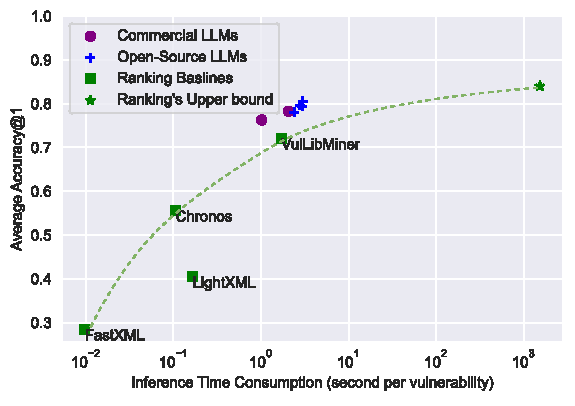
\includegraphics[width=1\linewidth]{figures/efficiency_accuracy_advanced.drawio.pdf}
\caption{Trade-Offs between Efficiency and Accuracy}
\label{fig: efficiency accuracy}
\vspace{-0.3cm}
\end{figure}


% \subsection*{\textbf{RQ3}: How efficient is \detector{} when compared with ranking approaches?}

% In this research question, we evaluate the efficiency of \detector{} when compared with both existing approaches and the estimated upper bound of ranking approaches. 

\noindent \textbf{Efficiency of Existing Work vs. \detector{}}. In Figure~\ref{fig: efficiency accuracy}, we visualize the actual computational cost and accuracy of each method in Table~\ref{tab: baseline cmp}. We further mark the upper bound of the ranking-based approach using LLMs for comparison. The Accuracy@1 is upper-bounded by the recall@512 of TF-IDF, i.e., the best possible Accuracy@1; while the time cost is upper-bounded by the time cost of invoking the 13B model 512 times (10 mins). 


We can observe the \detector{} achieves a sweet spot in the effectiveness and efficiency trade-off. When compared with existing work, \detector{} achieves a better Accuracy@1 while the time cost is comparable to the best-performed existing work~\cite{vullibminer}. When compared with the upper bound, \detector{} achieves a slightly lower Accuracy@1 while consuming less than 1/100 time and computation resources.
%The main reason is that VulLibMiner needs to invoke a lightweight model (BERT) multiple times (e.g., 512) while \detector{} needs to invoke LLMs only once. 

% In Figure~\ref{fig: efficiency accuracy}, additionally, we further mark the upper bound of the existing work for comparison. If we use the larger 13B model in the existing ranking-based approach, the Accuracy@1 is upper-bounded by the recall@512, i.e., assuming that a future model can perfectly order all top-512 packages; whereas the time cost upper-bounded by the time cost of invoking the 13B model 512 times (10 mins). When compared this the upper bound, \detector{} achieves a similar Accuracy@1 while consuming less than 1/100 time and computation resources. As a result, \detector{} achieves a sweet spot in the effectiveness and efficiency tradeoff. 



% \myfindings[1]{\detector{} is highly effective, achieving an average accuracy of 0.790 on four widely-used programming languages while the SOTA approaches achieve only 0.556.}




% \subsection*{\textbf{RQ2}: To what extent can our RAG technique and local search algorithm help generate vulnerable packages?}~\label{sec: rq2}
\subsection{Ablation Studies on \detector{}}
In this subsection, we conduct ablation studies on the three components of \detector{}: supervised fine-tuning, RAG, and local search.
% Additionally, we use Java vulnerabilities to evaluate whether the number and quality of our RAG packages affect the end-to-end effectiveness of \detector{}.

\noindent \textbf{SFT's Improvement}. By comparing the results of in-context learning vs supervised fine-tuning in Table~\ref{tab: baseline cmp}, we can see that SFT outperforms ICL by a larger margin.
%We observe that SFT also outperforms the baseline with neither ICL nor SFT, we have not shown the latter result due to space limit. 
This result indicates that for the 7B and 13B models, supervised fine-tuning on the full training data is essential in bridging the models' knowledge gap. 

% \subsubsection{Methodology}
% We evaluate the effectiveness of \detector{} with various recommended packages to see input augmentation's benefits on \detector{}.
% In this research question, we evaluate the base model of LLaMa-13B without unsupervised fine-tuning because its effectiveness is quite similar to other base models.
% Specifically, we use TF-IDF and VulLibMiner to recommend at most three packages.

\noindent \textbf{RAG's Overall Improvement:}
Table~\ref{tab: rag improvement} shows the improvement of our RAG technique in Accuracy@1.
Specifically, it improves the Accuracy@1 by 9.3\%, 1.8\%, 8.9\%, and 15.7\% on each programming language, respectively.
These improvements indicate that our RAG technique is effective in helping generate the names of vulnerable packages. 
We further report paired t-test results for Table~\ref{tab: rag improvement} in Table~\ref{tab: rag p value} of Appendix. 

Table~\ref{tab: rag improvement} also indicates that RAG's improvement in commercial LLMs is higher than that of open-source LLMs.
Especially in Go vulnerabilities, our RAG technique improves the Accuracy@1 by 57.6\% and 31.0\% on ChatGPT and GPT4.
The main reason is that both ChatGPT and GPT4 do not have sufficient domain knowledge about Go packages as they are relatively newer than packages of other programming languages~\cite{chatgpt_golang}. 
%Thus, RAG can guide these LLMs to generate a proper (existing) package name.

% of our RAG technique in Java vulnerabilities is higher than that in JS, Python, and Go vulnerabilities.
% The major reason is that the names of Java packages are more difficult to generate.
% Even if the improvement in Java is much higher than others, \detector{} still achieves the lowest Accuracy@1 in Java among four programming languages (as shown in Table~\ref{tab: baseline cmp}).

% \noindent \textbf{Difference Among Various Programming Languages}
% Table~\ref{tab: rag improvement} also indicates that the improvement of our RAG technique in Java vulnerabilities is higher than that in JS, Python, and Go vulnerabilities.
% The major reason is that the names of Java packages are more difficult to generate.
% Even if the improvement in Java is much higher than others, \detector{} still achieves the lowest Accuracy@1 in Java among four programming languages (as shown in Table~\ref{tab: baseline cmp}).



\begin{table}[t]
\centering
\small
\caption{RAG's Improvement ($Accuracy@1_{RAG} - Accuracy@1_{Raw}$)}
\label{tab: rag improvement}
\begin{tabular}{lrrrr}
\toprule
\multicolumn{1}{c}{\multirow{1}{*}{Language}} & \multicolumn{1}{c}{Java}                        &        \multicolumn{1}{c}{JS}                 &          \multicolumn{1}{c}{Python}               &     \multicolumn{1}{c}{Go}                    \\
\midrule
\multicolumn{3}{l}{\textit{Commercial LLMs:}}                          &                         &                         \\
ChatGPT                                       & 16.1\% $\uparrow$       & 3.6\% $\uparrow$       & 38.8\% $\uparrow$       & 57.6\% $\uparrow$                \\
GPT4                                          & 12.1\% $\uparrow$       &    0.9\% $\uparrow$                     &      0.9\% $\uparrow$                   &        31.0\% $\uparrow$                 \\ 
\midrule
\multicolumn{5}{l}{\textit{Full SFT on Open-Source LLMs:}}                                                                          \\
LLaMa-7B                                      & 2.2\% $\uparrow$       & 2.2\% $\uparrow$       & 3.1\% $\uparrow$       & 1.8\% $\downarrow$     \\
LLaMa-13B                                     & 3.3\% $\uparrow$       & 0.4\% $\uparrow$       & 2.0\% $\uparrow$       & 3.7\% $\uparrow$       \\
Vicuna-7B                                     & 13.6\% $\uparrow$      & 2.3\% $\uparrow$       & 3.8\% $\uparrow$       & 3.7\% $\uparrow$       \\
Vicuna-13B                                    & 8.7\% $\uparrow$      & 1.2\% $\uparrow$       & 4.9\% $\uparrow$       & 0.0\% -                \\
\midrule
Average                                      & 9.3\% $\uparrow$      & 1.8\% $\uparrow$       & 8.9\% $\uparrow$       & 15.7\% $\uparrow$         \\
\bottomrule
\end{tabular}
\vspace{-0.2cm}
\end{table}



\noindent \textbf{RAG Improvement vs. k/Retrieval Algorithm Choice}. We evaluate whether $k$ and the choice of retrieval algorithm affect the end-to-end effectiveness of \detector{}. Specifically, we focus on Java vulnerabilities (as Java package names are the most difficult to generate). 
The result can be found in Table~\ref{tab: various rag} in our Appendix.

For $k$, we conduct an Analysis of Variance (ANOVA)~\cite{anova} among the Accuracy@1 of six representative numbers of RAG packages (ranging from 1 to 20). Although $k=20$ has a slightly higher accuracy than $k=1$ for both TF-IDF and BERT, this difference is not significant. In fact, the paired t-test results show that there is no significant difference among the Accuracy@1 of different $k$ values ($p=0.814$ for TF-IDF and $p=0.985$ for BERT). 

As for the retrieval algorithm, we observe that Accuracy@1 with TF-IDF results is quite similar to that of non-RAG inputs, and the Accuracy@1 with BERT results is substantially higher than that of non-RAG/TF-IDF results. As a result, it is essential to use BERT-retrieved results in RAG. 


% We show that the Topk F1 scores on the full-shot testing set vary only a little upon different recommended packages.
% For example, the difference between the maximum and minimum values of F1@1 on the full-shot testing set is less than 0.04.
% On the contrary, the recommended packages substantially increase the F1@1 on the zero-shot testing set by 39\% (from 0.394 to 0.547).
% Additionally, recommended packages with higher quality (e.g., from no recommended packages to TF-IDF, or from TF-IDF to VulLibMiner) also help \detector{} to identify zero-shot packages.
% For example, the F1@1 increases by 8\% on average (upon Topk recommended packages) when we use the recommended results from VulLibMiner instead of TF-IDF.
% The main reason for this improvement is that zero-shot packages are difficult for LLMs to identify, and input augmentation provides examples of packages whose functionalities are likely to be affected by a given vulnerability.
% Thus, \detector{} can generate package names from those with similar functionalities instead of all packages.



% \begin{table*}[t]
% \centering
% \scriptsize
% \caption{Accuracy@1 with Various RAG Inputs in Generating the Names of Java Affected Packages}
% \label{tab: various rag}
% \begin{tabular}{llcccccccccccc}
% \toprule
% IR Model:      & None  & \multicolumn{6}{c}{TF-IDF Results}            & \multicolumn{6}{c}{BERT Results}              \\
% \cmidrule(lr){3-8}\cmidrule(lr){9-14}
% \multicolumn{2}{l}{\#RAG packages:} & 1                & 2               & 3     & 5       & 10      & 20      & 1               & 2              & 3     & 5       & 10      & 20      \\
% \midrule
% \multicolumn{3}{l}{\textit{Commercial LLMs:}}                    &                 &       &         &         &         &                 &                &       &         &         &         \\
% ChatGPT    & 0.597 & 0.523 & 0.498 & 0.508 & 0.552 & 0.540 & 0.567 & 0.758 & 0.743 & 0.722 & 0.718 & 0.715 & 0.710 \\
% GPT4       & 0.676 & 0.619 & 0.559 & 0.588 & 0.619 & 0.626 & 0.638 & 0.783 & 0.773 & 0.784 & 0.792 & 0.797 & 0.792 \\
% \midrule
% \multicolumn{5}{l}{\textit{Full SFT on Open-Source LLMs:}}                        &         &         &         &                 &                &       &         &         &         \\
% LLaMa-7B   & 0.688 & 0.692 & 0.697 & 0.701 & 0.563 & 0.591 & 0.609 & 0.710 & 0.701 & 0.710 & 0.678 & 0.665 & 0.683 \\
% LLaMa-13B  & 0.687 & 0.688 & 0.687 & 0.696 & 0.653 & 0.635 & 0.623 & 0.720 & 0.702 & 0.701 & 0.701 & 0.704 & 0.703 \\
% Vicuna-7B  & 0.561 & 0.596 & 0.398 & 0.404 & 0.441 & 0.439 & 0.421 & 0.697 & 0.701 & 0.683 & 0.685 & 0.706 & 0.683 \\
% Vicuna-13B & 0.623 & 0.609 & 0.450 & 0.418 & 0.650 & 0.655 & 0.680 & 0.710 & 0.712 & 0.701 & 0.722 & 0.719 & 0.720 \\
% \bottomrule
% \end{tabular}
% \vspace{-0.4cm}
% \end{table*}

\noindent \textbf{Local Search's Improvement}. 
Table~\ref{tab: post processing} shows the end-to-end 
improvement in Accuracy@1 of \detector{} before and after local search.
Our local search technique improves the Accuracy@1 by 3.43\%, 1.02\%, 1.57\%, and 6.20\% on each programming language. We further report paired t-test results for Table~\ref{tab: post processing} in Table~\ref{tab: local search p value} of Appendix. 

We make the following observations. First, local search is more effective on commercial LLMs (an average improvement of 4.58\%) than fine-tuned open-source LLMs (an average improvement of 2.29\%).
Since commercial LLMs are not fine-tuned, local search plays an important role in improving the effectiveness of generation. Second, local search is more effective on Java and Go than JS and Python. The reason is that since Java and Go packages are longer (8-14 tokens), LLMs are more prone to generating partially correct, non-existing outputs (i.e., Type 2 error in Table~\ref{tab: fault case study}).  Local search can effectively reduce this type of error. 

\begin{table}[t]
\centering
\small
\caption{Local Search's Improvement ($Accuracy@1_{Search} - Accuracy@1_{Raw}$)}
\label{tab: post processing}
\begin{tabular}{lrrrr}
\toprule
\multicolumn{1}{c}{\multirow{1}{*}{Language}} & \multicolumn{1}{c}{Java}                        &        \multicolumn{1}{c}{JS}                 &          \multicolumn{1}{c}{Python}               &     \multicolumn{1}{c}{Go}                    \\
\midrule
\multicolumn{3}{l}{\textit{Commercial LLMs:}}                          &                         &                         \\
ChatGPT                                       & 4.1\% $\uparrow$       & 1.2\% $\uparrow$       & 0.7\% $\uparrow$       & 11.1\% $\uparrow$                \\
GPT4                                          & 5.3\% $\uparrow$       &    2.5\% $\uparrow$                     &      2.9\% $\uparrow$                   &        8.8\% $\uparrow$                 \\ 
\midrule
\multicolumn{5}{l}{\textit{Full SFT on Open-Source LLMs:}}                                           \\
LLaMa-7B                                      & 2.9\% $\uparrow$       & 0.9\% $\uparrow$       & 2.2\% $\uparrow$       & 7.0\% $\uparrow$     \\
LLaMa-13B                                     & 3.3\% $\uparrow$       & 0.3\% $\uparrow$       & 0.7\% $\uparrow$       & 4.1\% $\uparrow$       \\
Vicuna-7B                                     & 3.9\% $\uparrow$      & 0.9\% $\uparrow$       & 1.8\% $\uparrow$       & 3.3\% $\uparrow$       \\
Vicuna-13B                                    & 1.1\% $\uparrow$      & 0.3\% $\uparrow$       & 1.1\% $\uparrow$       & 2.9\% $\uparrow$       \\
\midrule
Average                                      & 3.4\% $\uparrow$      & 1.0\% $\uparrow$       & 1.4\% $\uparrow$       & 6.2\% $\uparrow$         \\
\bottomrule
\end{tabular}
% \vspace{-0.4cm}
\end{table}

% \subsection*{\textbf{RQ3}: How efficient is \detector{} when compared with ranking approaches?}

% In this research question, we evaluate the efficiency of \detector{} when compared with both existing approaches and the estimated upper bound of ranking approaches. 

% \noindent \textbf{Trade-Offs between Effectiveness and Efficiency:}
% It is shown in Figure~\ref{fig: efficiency accuracy}.
% When compared with the SOTA ranking baselines, \detector{} achieves better Accuracy@1  while keeping similar time consumption.
% The main reason is that VulLibMiner needs to invoke a lightweight model (BERT) multiple times (e.g., 512) while \detector{} needs to invoke LLMs only once, thus indicating the effectiveness of replacing ranking with generation.

% Additionally, we also mark the upper bound of ranking approaches for comparison.
% Its time consumption is estimated by invoking Vicuna-13B 512 times, and its Accuracy@1 is estimated as the recall@512 of VulLibMiner, i.e., assuming that a future model can correctly order all candidate packages.
% When compared with the upper bound of ranking approaches, \detector{} achieves similar Accuracy@1 while consuming less than 1/100 time and computation resources.

% \begin{figure}[t]
% \centering
% 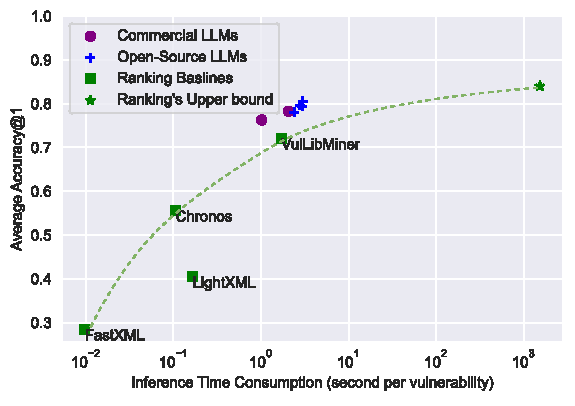
\includegraphics[width=1\linewidth]{figures/efficiency_accuracy_advanced.drawio.pdf}
% \caption{Trade-Offs between Efficiency and Accuracy}
% \label{fig: efficiency accuracy}
% \end{figure}


% \noindent \textbf{The Effectiveness of Constrained Decoding:}
% Table~\ref{tab: post processing} shows the end-to-end Accuracy@1 of \detector{} before and after constrained decoding on open-source LLMs.
% For each combination of programming language and open-source LLMs, constrained decoding improves the end-to-end Accuracy@1 by x.xx\% on average.




% \begin{table}[t]
% \centering
% \small
% \caption{Time Consumption Per Vulnerability}
% \label{tab: time consumption}
% \begin{threeparttable}
% \begin{tabular}{lcccc}
% \toprule
% \multicolumn{1}{c}{\multirow{1}{*}{}} & \multicolumn{1}{c}{\makecell[c]{None}}                        &        \multicolumn{1}{c}{\makecell[c]{Hard\\ Constraints}}                             &     \multicolumn{1}{c}{\makecell[c]{Bigram\\ Constraints}}                    \\
% \midrule
% LLaMa-7B   & 2.41s    & >2h            & 9.48s \\
% LLaMa-13B  & 2.78s    & >2h            & 15.71s \\
% Vicuna-7B  & 2.95s    & >2h            & 9.86s \\
% Vicuna-13B & 3.01s    & >2h            & 15.71s \\
% \midrule
% Average    & 2.79s    & >2h            & 15.71s \\
% \bottomrule
% \end{tabular}
% % \begin{tablenotes}
% %     \footnotesize
% %     \item Column ``All packages'' and ``Top512 packages'' refer to constrained decoding with hard constraints.
% % \end{tablenotes}
% \end{threeparttable}
% \end{table}




% \subsection*{\textbf{RQ4}: How much benefit can security practice gain from our approach?}
% \vspace{-0.2cm}
\subsection{Evaluating \detector{} Performance in Real World Setting}~\label{sec: real world}
% \vspace{-0.4cm}

\noindent To examine \detector{}'s performance in the real-world setting, for each programming language, we randomly sample and report a subset of <vulnerability, affected package> pairs that are not listed in GitHub Advisory (Java: 25, JS: 14, Python: 11, Go: 10). 
We use \detector{} to generate the package names and submit the generated names (\detector{} with Vicuna-13B) to GitHub Advisory. 
% \xueqing{fill xxx with the exact setting in Table 3}. 

At the time of the writing,  the results are summarized below. \textbf{Java}: 21 of them have been accepted and merged into GitHub Advisory. Among the remaining 4 packages, 2 of them are considered non-vulnerabilities, and 2 of them are considered incorrect affected packages. \textbf{JS, Python, and Go}: 13 of them have been accepted and merged into GitHub Advisory (2 JS, 8 Python, 3 Go). The details of these packages are listed in Table~\ref{tab: github issue} of Appendix. 

This result highlights the real-world performance of \detector{} in automatically identifying affected package names. 


% To evaluate \detector{}'s impact on our security practice, we take \detector{} as an oracle to identify <vulnerability, package> pairs as complements of one open-sourced vulnerability database, GitHub Advisory~\cite{githubAD}.
% Note that there are a large amount of Java vulnerabilities besides those included in VulLib and the number of vulnerabilities is rapidly increasing. In this research question, we conduct an empirical study by answering the following two sub-questions:


% \myfindings[4]{\detector{} substantially reduces the manual costs of identifying the affected packages of vulnerabilities.
% Additionally, we demonstrate \detector{}'s high value of security practice by submitting 25 of the identified <vulnerability, package> pairs to GitHub Advisory, and 22 of them are accepted.}


% \begin{table}[t]
% \centering
% \small
% \caption{Constrained Decoding's Improvement in Accracy@1 }
% \label{tab: constrained decoding}
% \begin{tabular}{lcccc}
% \toprule
% \multicolumn{1}{l}{\multirow{1}{*}{Language}} & \multicolumn{1}{c}{Java}                        &        \multicolumn{1}{c}{JS}                 &          \multicolumn{1}{c}{Python}               &     \multicolumn{1}{c}{Go}                    \\
% \midrule
% % \multicolumn{5}{l}{\textit{Existing/non-existing package names:}}                         \\
% %  % & 3.38:1       & 20:1       & 20:1        & 2:1     \\
% % % \midrule
% $\lambda_{LLM}: \lambda_{trie}$ & 5:1       & 20:1       & 20:1        & 5:1     \\
% \midrule
% % LLaMa-7B                         & 2.3\% $\uparrow$      & 0.3\% $\uparrow$       & 1.1\% $\uparrow$       & 2.9\% $\uparrow$       \\
% % LLaMa-13B                         & 2.4\% $\uparrow$      & 0.3\% $\uparrow$       & 1.1\% $\uparrow$       & 2.9\% $\uparrow$       \\
% Vicuna-7B                         & 2.4\% $\uparrow$      & 1.5\% $\downarrow$       & 0.5\% $\uparrow$       & 2.2\% $\uparrow$       \\
% Vicuna-13B                         & 1.9\% $\uparrow$      & 0.1\% $\downarrow$       & 1.1\% $\uparrow$       & 2.9\% $\uparrow$       \\
% \bottomrule
% \end{tabular}
% \end{table}




% \begin{table}[t]
% \centering
% \small
% \caption{Constrained Decoding's Improvement (Accuracy@1)}
% \label{tab: constrained decoding}
% \begin{tabular}{lcccc}
% \toprule
% \multicolumn{1}{c}{\multirow{1}{*}{Language}} & \multicolumn{1}{c}{Java}                        &        \multicolumn{1}{c}{JS}                 &          \multicolumn{1}{c}{Python}               &     \multicolumn{1}{c}{Go}                    \\
% \midrule
% \multicolumn{5}{l}{\textit{Existing/non-existing package names:}}                         \\
%  % & 3.38:1       & 20:1       & 20:1        & 2:1     \\
% % \midrule
% $\lambda_{LLM}: \lambda_{trie}$ & 3:1       & 20:1       & 20:1        & 2:1     \\
% \midrule
% LLaMa-7B                         & 2.25\% $\uparrow$      & 0.3\% $\uparrow$       & 1.1\% $\uparrow$       & 2.9\% $\uparrow$       \\
% LLaMa-13B                         & 2.25\% $\uparrow$      & 0.3\% $\uparrow$       & 1.1\% $\uparrow$       & 2.9\% $\uparrow$       \\
% Vicuna-7B                         & 2.25\% $\uparrow$      & 0.3\% $\uparrow$       & 1.1\% $\uparrow$       & 2.9\% $\uparrow$       \\
% Vicuna-13B                         & 2.25\% $\uparrow$      & 0.3\% $\uparrow$       & 1.1\% $\uparrow$       & 2.9\% $\uparrow$       \\
% \bottomrule
% \end{tabular}
% \end{table}


% \begin{table}[t]
% \centering
% \small
% \caption{Time Consumption of Constrained Decoding per Vulnerability}
% \label{tab: time consumption}
% \begin{threeparttable}
% \begin{tabular}{lcccc}
% \toprule
% \multicolumn{1}{c}{\multirow{1}{*}{}} & \multicolumn{1}{c}{\makecell[c]{None}}                        &        \multicolumn{1}{c}{\makecell[c]{All\\ Packages}}                 &          \multicolumn{1}{c}{\makecell[c]{Top512\\ Packages}}               &     \multicolumn{1}{c}{\makecell[c]{Bigram}}                    \\
% \midrule
% LLaMa-7B   & 2.41s    & >2h          & 81.91s          & 15.71s \\
% LLaMa-13B  & 2.78s    & >2h          & 81.91s          & 15.71s \\
% Vicuna-7B  & 2.78s    & >2h          & 81.91s          & 15.71s \\
% Vicuna-13B & 2.78s    & >2h          & 81.91s          & 15.71s \\
% \midrule
% Average    & 2.78s    & >2h          & 81.91s          & 15.71s \\
% \bottomrule
% \end{tabular}
% \begin{tablenotes}
%     \footnotesize
%     \item Column ``All packages'' and ``Top512 packages'' refer to constrained decoding with hard constraints.
% \end{tablenotes}
% \end{threeparttable}
% \end{table}






% \begin{table*}[t]
% \centering
% \caption{Accuracy@1 with Various Techniques to Address Outputs of Non-Existing Packages}
% \label{tab: post processing}
% \begin{tabular}{lccccccccc}
% \toprule
%            & \multicolumn{3}{c}{Java}                         & \multicolumn{2}{c}{JS}    & \multicolumn{2}{c}{Python} & \multicolumn{2}{c}{Go}    \\
% \cmidrule(lr){2-4}\cmidrule(lr){5-6}\cmidrule(lr){7-8}\cmidrule(lr){9-10}
%            & \makecell[c]{Raw\\ Output} & \makecell[c]{Local\\ Search} & \makecell[c]{Constrained\\ Decoding} & \makecell[c]{Raw\\ Output} & \makecell[c]{Local\\ Search} & \makecell[c]{Raw\\ Output} & \makecell[c]{Local\\ Search} & \makecell[c]{Raw\\ Output} & \makecell[c]{Local\\ Search} \\
% \midrule
% \multicolumn{10}{l}{\textit{Commercial LLMs:}}                                                                                                               \\
% ChatGPT    & 0.717      & 0.758        & -                    & 0.720      & 0.732        & 0.908       & 0.915        & 0.535      & 0.646        \\
% GPT4       & 0.744      & 0.797        & -                    &     0.743       &       0.768       &    0.839         &     0.868         &    0.624        &       0.712       \\
% \midrule
% \multicolumn{10}{l}{\textit{Open-Source LLMs:}}                                                                                                              \\
% LLaMa-7B   & 0.681 & 0.710 & 0.733 & 0.764 & 0.773 & 0.902 & 0.924 & 0.646 & 0.716 \\
% LLaMa-13B  & 0.687 & 0.720 & 0.744 & 0.762 & 0.765 & 0.897 & 0.904 & 0.734 & 0.775 \\
% Vicuna-7B  & 0.658 & 0.697 & 0.721 & 0.759 & 0.768 & 0.911 & 0.929 & 0.749 & 0.782 \\
% Vicuna-13B & 0.699 & 0.710 & 0.729 & 0.770 & 0.773 & 0.924 & 0.935 & 0.775 & 0.804 \\
% \bottomrule
% \end{tabular}
% \end{table*}


% \section{Threats to Validity} \label{sec:threats}

A major threat to external validity is that the maven corpus we used during post-processing does not include all Java libraries.
This corpus contains Java libraries and descriptions until 2022, so new libraries or private ones are not contained in this corpus and cannot be generated by \detector{}.
This threat could be reduced by extending this corpus with the libraries used by the developers themselves.
The threats to internal validity are instrumentation effects that can bias our results. Faults in our tool or its underlying third-party tools (e.g., the entity-linking approaches for library recommendation) might cause such effects. 
To reduce these threats, we manually inspect the intermediate results to make sure that the accuracy of their recommended libraries is quite similar to the reported values in their paper~\cite{vullib}.


\input{related}
% \detector{} also includes the input augmentation technique to help identify zero-shot vulnerable libraries (those not occurring during training) and the post-processing technique to help address \detector{}'s hallucinations. 
% We have conducted a comprehensive evaluation of demonstrating \detector{}'s effectiveness in identifying vulnerable libraries with an average F1 score of 0.626 while the state-of-the-art/practice approaches achieve only 0.561. 
% We have demonstrated the effectiveness of the post-processing technique with an average improvement of F1@1 by 9.3\%, and the effectiveness of the input augmentation technique with an average improvement of F1@1 by 39\% in identifying zero-shot libraries.

% adding recommended libraries with an average improvement of F1@1 by 38\% in identifying zero-shot libraries.
% We have shown the effectiveness of post-processing by improving the average F1@1 by 9.3\%.


% In this paper, we have presented our work, being the first to model vulnerable-library identification as an entity-link task and to identify zero-shot libraries.   
% We have designed a coarse-grained TF-IDF matcher to efficiently screen out a set of candidate libraries and a fine-grained BERT-FNN model to effectively identify the affected libraries for a given vulnerability.
% We have constructed a new dataset that is manually labeled and validated by senior software engineers, including 2,789 Java vulnerabilities and 324 negative samples.    
% We have conducted a comprehensive evaluation of demonstrating \detector{}'s effectiveness and efficiency for library identification, achieving an average F1 score of 0.542, while the state-of-the-art/practice approaches achieve only 0.377. We have demonstrated  \detector{}'s high value of security practice by using \detector{} to identify a new set of 7,936 <vulnerability, library> pairs for Java, which do not appear yet in NVD's existing 4,780 pairs for Java.

% \vspace{-0.15cm}

% \section{Data Availability}
% We list 225 <vulnerability, library> pairs to show high value of security practice on our anonymous website~\cite{repo}.
% We plan to open-source our  \javadata{} dataset, and all evaluation results at the publication of our paper. 
% We do not open-source our code repository now due to the security requirement of our industry partner.
% However, in Section~\ref{sec:approach}, we list all details of our approach, so that our approach can be easily reproduced.

\section{Conclusion}\label{sec:conclusion}
In this paper, we have proposed \detector{}, the first framework for identifying vulnerable packages using LLM generation. \detector{} conducts retrieval-augmented generation, supervised fine-tuning, and a local search technique to improve the generation. \detector{} is highly effective, achieving an accuracy of 0.806 while the best SOTA approaches achieve only 0.721.
\detector{} has shown high value to security practice. 
We have submitted 60 pairs of <vulnerability, affected package> to GitHub advisory and 34 of them have been accepted and merged. 
% \newpage


\section{Limitation}~\label{sec: limitation}
Our work has several limitations, which we plan to address in our future work:

\noindent \textbf{Challenges in Generating Long and Complex Package Names}. 
As discussed in Section~\ref{sec: trade off}, the effectiveness of \detector{} depends on the token length and the number of unique packages.
Table~\ref{tab: baseline cmp} shows Java is more challenging than others while having the highest token length and unique packages (Table~\ref{tab: dataset info}). 
%Vicuna-13B's Accuracy@1 in Java vulnerabilities (0.710) is less than that of Python vulnerabilities (0.935).
To improve the generation of complicated languages such as Java, we plan to further enhance the knowledge of LLM using techniques such as constrained decoding~\cite{post-vilar-2018-fast}. We leave this as our future work.
% two main features of package names, the number of unique packages in the dataset and the average token number of packages.
% Thus, exploring how to generate longer package names or how to generate package names from a limited number of training data is the future work of this paper.
In particular, it may pose further challenges to generate packages that are exceptionally long. To understand the distribution of token lengths, we report the quantile statistics of the token lengths in Table~\ref{tab: quantile} of Appendix. Table~\ref{tab: quantile} shows that the majority of the package names are shorter than 20 tokens, therefore, exceptionally long package names are very rare. 

\noindent \textbf{Challenges in Generating Package Names with Limited Ecosystem Knowledge}. 
Though \detector{} has demonstrated its effectiveness in four widely-used programming languages, some other programming languages, e.g., C/C++, do not have a commonly used ecosystem that maintains all its packages.
Thus, it is difficult to generate/retrieve the affected packages of C/C++ vulnerabilities as we do not have specific ranges during the RAG step of \detector{}.
Exploring how to generate RAG results without a commonly used ecosystem (e.g., Maven or Pypi) or collecting other useful information for RAG is the future work of this paper.

% \noindent \textbf{Future Work on Deploying \detector{} in Real World Settings.}
% In Section~\ref{sec: real world}, we deploy \detector{} to generate the names of 28 affected Java packages (4 of them are JS). 
% %, and 4 of these are actually JavaScript (because JS packages are also treated as Java, e.g., "jquery" is also treated as "org.webjars.npm:jquery").
% We focus on Java for two main reasons.
% First, the submission to GitHub advisory requires domain expertise for validating the generated results, and our author team has the best expertise in Java.
% Second, \detector{} was first designed and experimented for the Java dataset (VulLib) before extended to the other three programming languages.
% We plan to also submit the other programming languages in future work.
% We project similar acceptance rates as Java, since the platform, submission process, and \detector{}'s performance are all similar (or even higher).


\section{Ethical Consideration}

\noindent \textbf{License/Copyright.}
\detector{} utilizes open-source data from GitHub Advisory, along with four third-party package ecosystems.
We refer users to the original licenses accompanying the resources of these data.

\noindent \textbf{Intended Use.}
\detector{} is designed as an automatic tool to assist maintainers of vulnerability databases, e.g., GitHub Advisory.
Specifically, \detector{} helps generate the names of affected packages to complement the missing data of these databases.
The usage of \detector{} is also illustrated in Section~\ref{sec:approach} and our intended usage of \detector{} is consistent with that of GitHub Advisory~\cite{githubAD}.

\noindent \textbf{Potential Misuse.}
Similar to existing open-source LLMs, one potential misuse of \detector{} is generating harmful content.
Considering that we use open-source vulnerability data for LLM fine-tuning, the LLM might view harmful content during this step.
To avoid harmful content, we use only reviewed vulnerability data in GitHub Advisory, so such misuse will unlikely happen. 
Overall, the scientific and social benefits of the research arguably outweigh the small risk of their misuse.



% \xueqing{Unify the format of the reference, e.g., URL}


% Though \detector{} has demonstrated its effectiveness in four widely-used programming languages, some other programming languages, e.g., C/C++, do not have a commonly used ecosystem that maintains all its packages.
% Thus, it is difficult to generate/retrieve the affected packages of C/C++ vulnerabilities as we do not have specific ranges during the RAG step of \detector{}.
% Exploring how to generate RAG results without a commonly used ecosystem (e.g., Maven or Pypi) or collecting other useful information for RAG is the future work of this paper.



% \subsubsection*{\textbf{Identifying vulnerable libraries of other programming languages}}
% \detector{} is generalizable enough because it does not depend on specific characteristics of Java vulnerabilities.
% Take Python as an example programming language, \detector{} can identify the affected libraries after training on a dataset of Python <vulnerability, library> pairs, and the recommended libraries can be generated by entity-linking approaches with the descriptions of Python libraries (e.g., those collected from PyPI~\cite{pypi}).
% We implement and evaluate \detector{} on Java vulnerabilities because vulnerable Java libraries are difficult to identify due to their large scale and complicated structures.
% Another reason is that Java libraries are widely used in software development~\cite{wang2020empirical}, thus indicating the importance of identifying vulnerable Java libraries.

 
% \subsubsection*{\textbf{Larger pre-trained language models}}
% Although we expect that the larger, even commercial LLMs can be more effective in identifying vulnerable libraries.
% First and most pragmatically, these larger models lead to higher training and prediction cost of GPU resources and energies, thus increasing the usage burden in practice.
% And from a scientific perspective, the evaluation results of a 7B/13B model are sufficient to show the effectiveness of \detector{}, and its components.
% As shown in Section~\ref{sec: rq1}, there is no substantial difference between the F1@1 of 7B and 13B models.
% Thus, LLaMa-7B and LLaMa-13B are suitable for this task.


% We do admit that larger LLMs might increase the effectiveness of identifying vulnerable libraries; however, training and inference on these larger models 
% The answer to this question is no because complicated deep-learning models are computationally more expensive and require larger training sets~\cite{thompson2020computational}.
% As shown in Section~\ref{sec: rq4}, there are 310,844 Java libraries with only 12,716 <vulnerability, library> pairs
% Considering the imbalance of the large number of libraries and the small number of <vulnerability, library> pairs for training, a BERT-FNN model is suitable for this task.


% Taking Java vulnerabilities as an example, there are 310,844 Java libraries with only 12,716 <vulnerability, library> pairs.
% Even if we manually label all the CVEs, the number of libraries with various programming languages is still larger than <vulnerability, library> pairs.


\bibliographystyle{acl_natbib}
\bibliography{sample-base}
\input{appendix}

\end{document}
